%!TEX root = ../main.tex

\chapter{Architettura del sistema}

Chiariamo come prima cosa la differenza tra un antenna per la televisione satellitare e un'antenna Starlink.
Le parabole TV utilizzano un riflettitore parabolico per focalizzare le onde elettromagnetiche che costituiscono i segnali televisivi inviati dai satelliti di trasmissione in orbita attorno alla terra e un'altitudine di 35'000 km.
Le parabole TV ricevono solo segnali televisivi dallo spazio, non possono inviare dati.
La parabola Starlink, invece, invia e riceve dati Internet da un satellite starlink in orbita a 550km di distanza.
I fasci tra la parabola Starlink e il satellite deovno essere concentrati in fasci potenti e stretti, continuamente orientati per puntare l'uno verso l'altro \cite{branch_education_how_2022}.
Attualmente ci sono 6398 satelliti Starlink in orbita \cite{jonathan_mcdowell_starlink_nodate}.

\begin{figure}[ht]
  \centering
  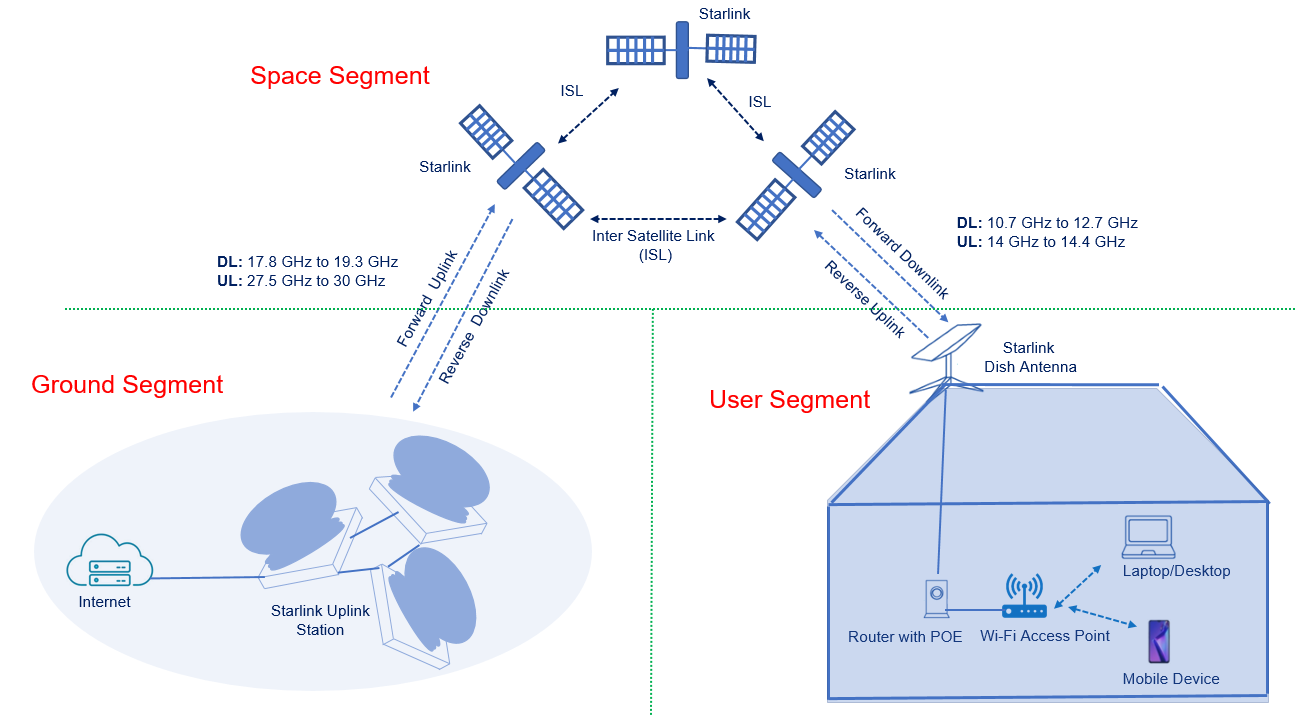
\includegraphics[width=0.9\linewidth]{./res/img/starlink-system-architecture.png}
  \caption{Architettura di sistema \cite{techplayon_spacex_2024}}
  \label{fig:starlink-system-architecture}
\end{figure}

\section{Segmento spaziale}
Questo segmento è costituito da un numero di satelliti in \ac{LEO}. Si tratta di piccoli satelliti a basso costo che pesano circa 260kg (nella versione 1.0), operano in \ac{Ku} e \ac{Ka} band e hanno durata di vita di 5-7 anni. \cite{techplayon_spacex_2024} Questi satelliti collegano l'utente a Internet.

Poichè esiste un numero enorme di satelliti questi comunicano tra loro attraverso \ac{LISL}, cioè una tecnologia ottica nello spazio libero.
I \ac{LISL} facilitano la trasmissione di dati ad alta velocità tra satelliti in una costellazione, e sono cruiciali per la rete Starlink per andare incontro alla crescente domanda di comunicazioni a bassa latenza ed alta capacità.
Adottare \ac{LISL} ha dei vantaggi rispetto ai classici collegamenti a radiofrequenza (\ac{RF}).
\begin{itemize}
  \item Data rate più alti dato che si usano laser invece di link \ac{RF}.
  \item Dimensione e peso minore dato che l'utilizzo di laser consente di avere antenne più piccole, risultando in un peso e volume ridotto per i terminali di comunicazione, rendendoli più semplici da integrare nei satelliti.
  \item Migliore sicurezza dato che l'ampiezza ridotta del fascio laser riduce al minimo le interferenze e migliora la sicurezza rendendo più difficile l'intercettazione del segnale.
  \item Basso consumo energetico della tecnologia laser.
\end{itemize}

I satelliti Starlink saranno equipaggiati con quattro terminali \ac{LISL} ciascuno, per consentire comunicazioni con satelliti vicini nello stesso piano orbitale e in piani orbitali adiacenti.
\begin{itemize}
  \item \ac{LISL} intra-orbitali:
  \item \ac{LISL} inter-orbitali:
\end{itemize}

\section{Segmento di terra}
I segmenti di terra includono diverse facilities che gestiscono la rete e forniscono connettività internet ai satelliti. Questi funzionano anche da Graund Station e sono localizzati strategicamente intorno al mondo per fornire copertura a zone remote e con poca connettività a internet.
La ground station è connessa all'\ac{ISP} tramite fibra.\cite{branch_education_how_2022}

\section{Segmento utente}
Il segmento utente comprende l'area in cui le persone utilizzano i servizi internet tramite il kit che viene fornito e che comprende l'antenna per la trasmissione, il cavo di alimentazione, il router (tranne nella versione mini dell'antenna dove il router è integrato all'antenna) e il cavo di rete per connettere l'antenna al router se quest'ultimo è incluso.\cite{branch_education_how_2022}

\subsection{Antenna}

\subsubsection{Struttura generale}
Aprendo la parabola (versione 1.0 revisione 2) troviamo sul retro una coppia di motori e un cavo ethernet che si collega al router.
Questi motori non muovono continuamente la parabola per puntare direttamente al satellite con cui comunica; vengono utilizzati solo durante la configurazione iniziale per orientare l'antenna nella direzione generale corretta.
Aprendo la parabola troviamo una piastra posteriore strutturale in alluminio e, dall'altro lato, una grande scheda a circuiti stampati (PCB).
Su un lato ci sono 640 microchip piccoli e 20 microchip più grandi, disposti in un pattern con tracce che si diramano dai microchip più grandi a quelli più piccoli, insieme a chp aggiuntivi, inclusa la CPU principale e il modulo GPS sul bordo del PCB. Sull'altro lato cisono circa 1'400 cerchi di rame con una griglia di quadrati tra i cerchi.
Nel livello successivo c'è uno schema a nido d'ape in gomma con piccoli cerchi di rame intagliati e dietro troviamo un altro schema a nido d'ape e poi la copertura anteriore della parabola.
Abbiamo quindi 1280 antenne disposte in un pattern esagonale a nido d'ape, con ciascuna pila di cerchi di rame che rappresenta una singola antenna controllata dai microchip sul PCB.
Questo enorme array funziona insieme in quella che è chiamata un'antenna phased array per inviare e ricevere onde elettromagnetiche che vengono direzionate verso e da un satellite Starlink in orbita a 550km di distanza.\cite{branch_education_how_2022}

\subsubsection{Funzionamento dell'antenna Aperture Couple Patch}

\begin{figure}[htbp]
  \centering
  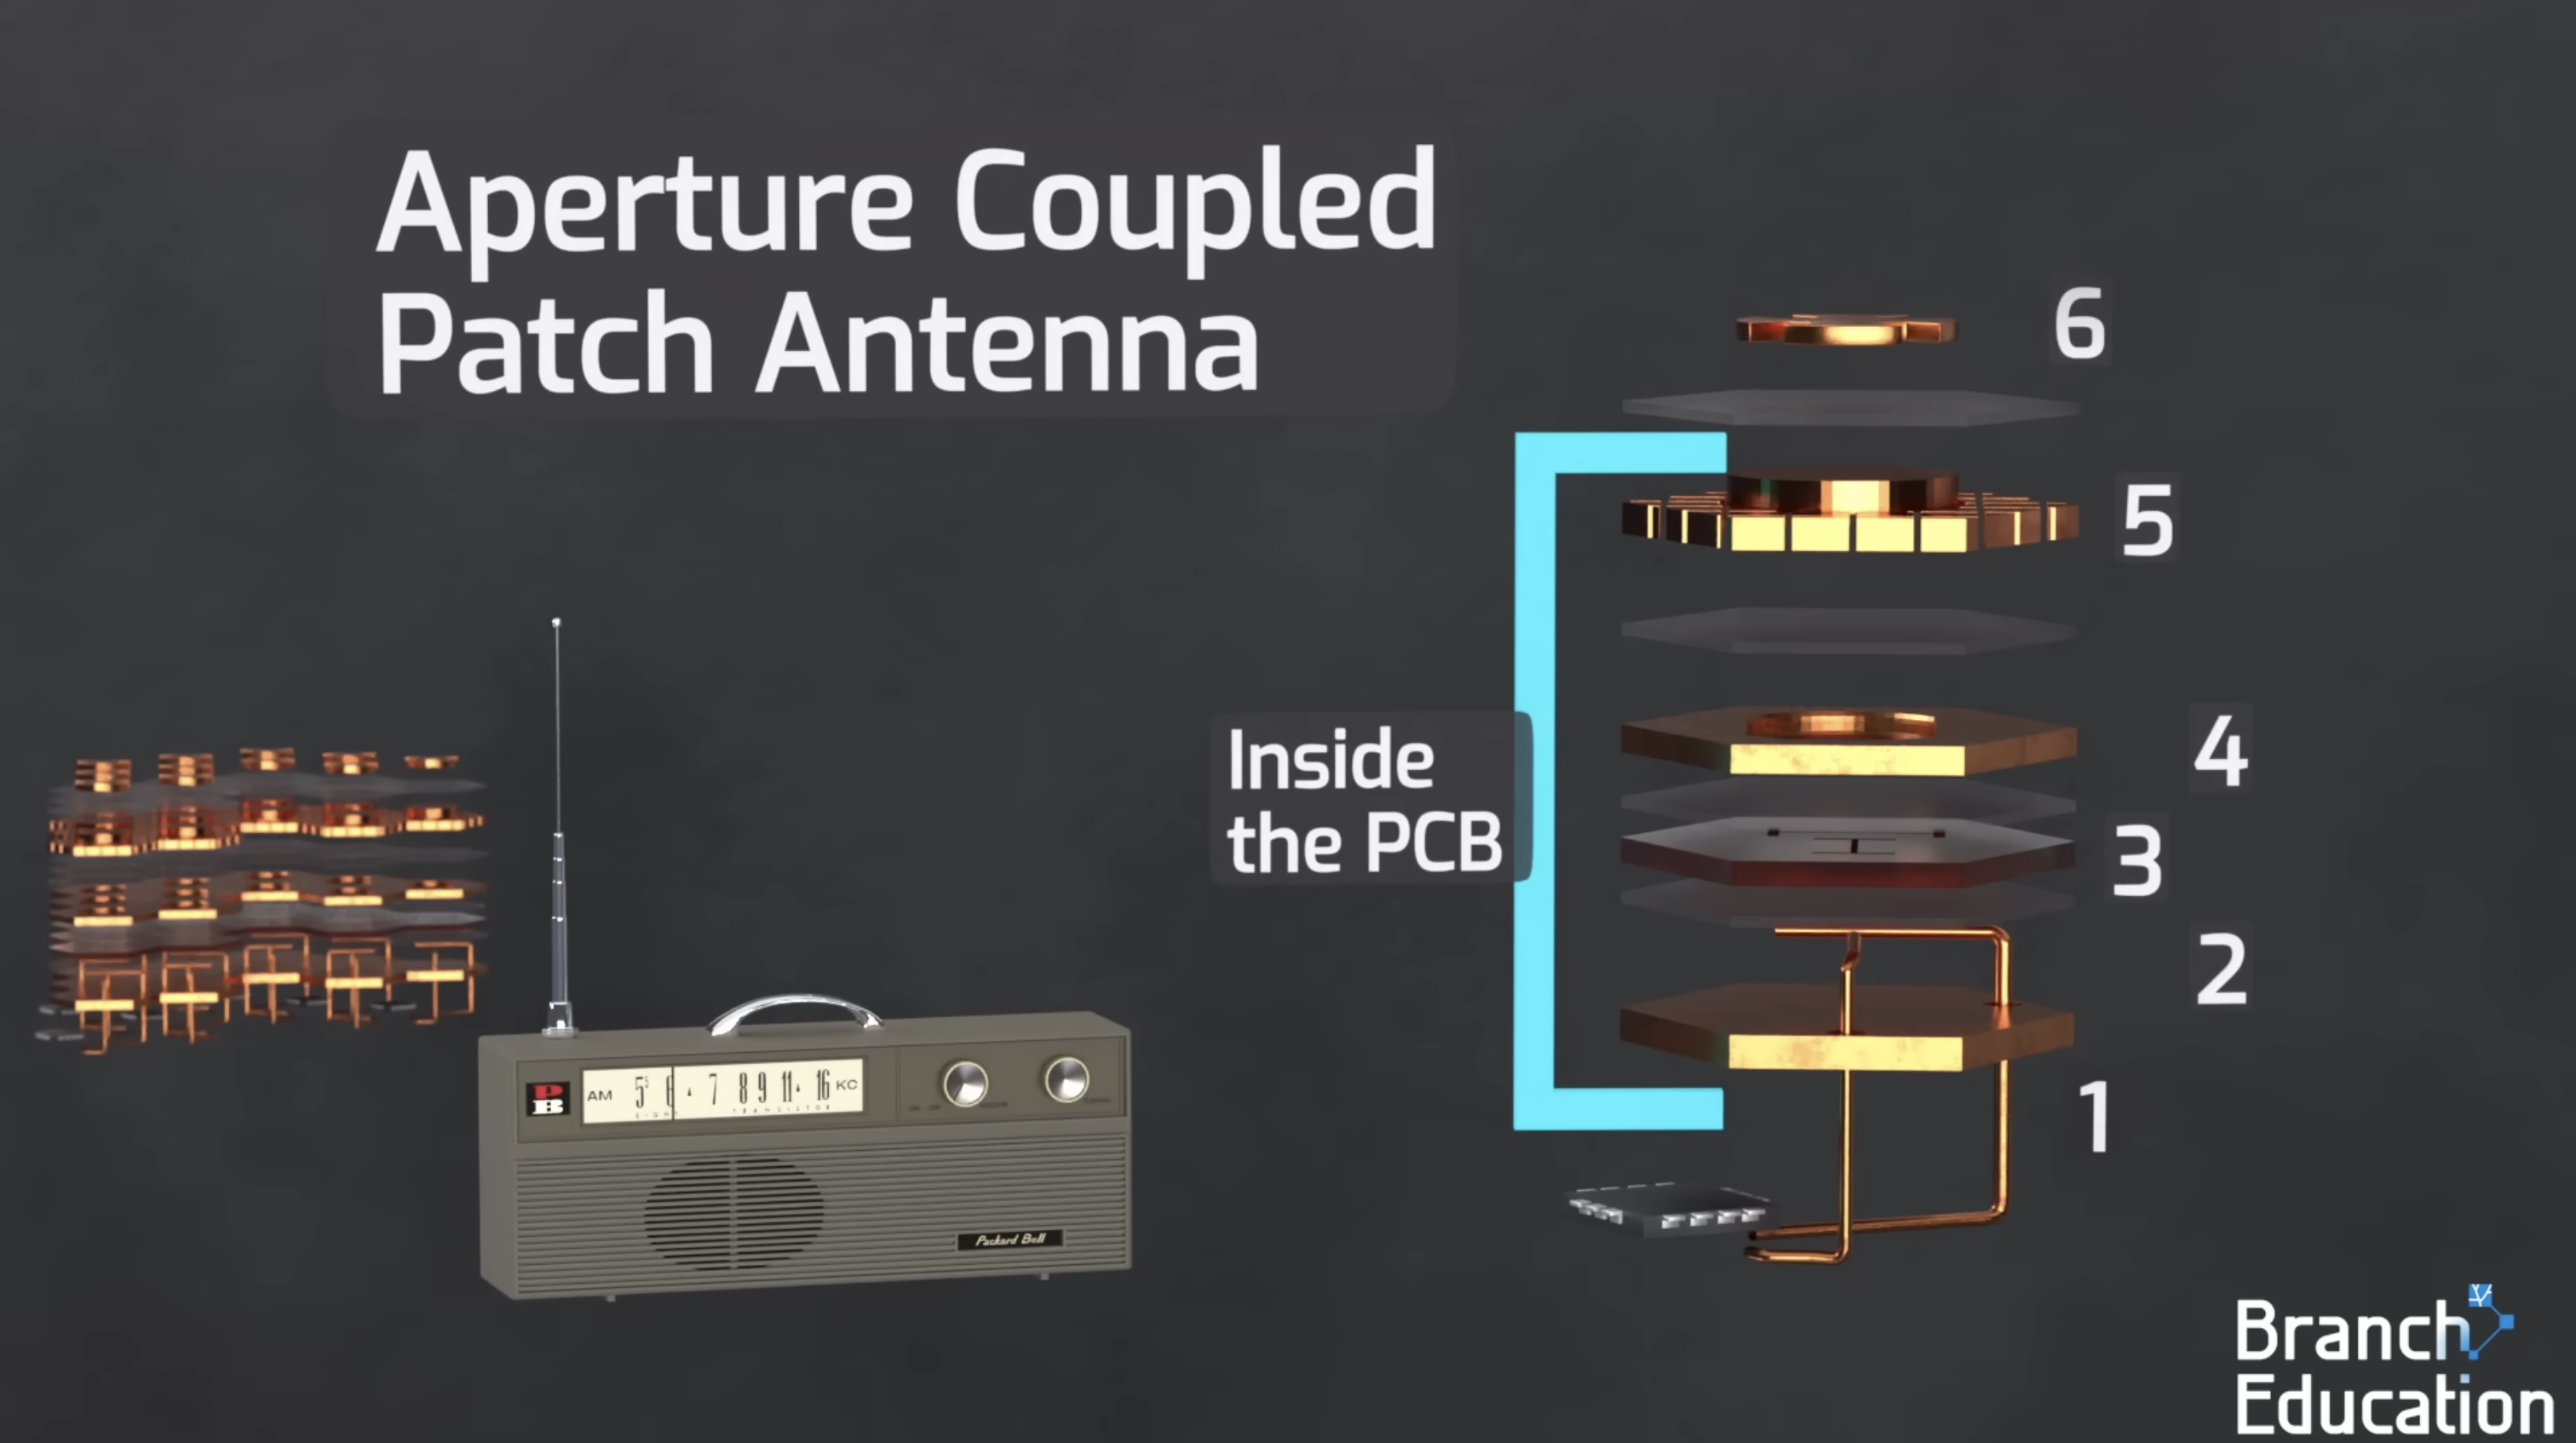
\includegraphics[width=0.8\linewidth]{./res/img/antenna_pcb.png}
  \caption{Aperture Couple Patch antenna \cite{branch_education_how_2022}}
  \label{fig:aperture-couple-patch-antenna}
\end{figure}

Nella figura \ref{fig:aperture-couple-patch-antenna} possiamo vedere un'aperture couple patch antenna, composta di 6 layer, il più dei quali all'interno del PCB.
I layer più importanti sono:
\begin{itemize}
  \item[1] linea di alimentazione.
  \item[2] piano RF reflective.
  \item[3] H slot per la polarizzazione.
  \item[4] isolamento dell'antenna.
  \item[5] Bottom antenna patch: trasmettitore a 13 GHz.
  \item[6] Top antenna patch: ricevitore a 11.7 GHz.
\end{itemize}
I pezzi esagonali grigio scuro invece sono isolamento elettrico tra i vari layer.\cite{branch_education_how_2022}

Per facilitare la comprensione del suo funzionamento semplifichiamola rimuovendo per il momento alcuni layer per semplificare la sua comprensione, e vediamo i principi base di come si genera un'onda elettromagnetica che si propaga da quest'antenna.

Per iniziare, sul fondo abbiamo una micro linea di trasmissione elettrica che arriva da uno dei piccoli microchip.
Questa linea di trasmissione è solo un filo di rame che termina sotto la pila dell'antenna.
Mandiamo una tensione sinusodiale alla frequenza di 12 GHz al filo di alimentazione, che vuol dire che il segnale passa da positivo a negativo ogni 83 pico secondi.
Al di sopra del filo di rame di alimentazione abbiamo un cerchio di rame con intagli chiamato patch d'antenna.

Con la corrente continua o alternata a bassa frequenza, non succederebbe molto perchè il patch è isolato, ma con un segnale ad alta frequenza la potenza inviata al filo di alimentazione viene accoppiata o inviata al patch.
Questo fenomeno avviene perchè quando la tensione è al fondo della sua sinusoide, o al minimo, c'è una concentrazione di elettroni spinti verso l'estremità del filo di alimentazione, creando così una zona di carica negativa che corrisponde alla massima tensione negativa.
Questa concentrazione di elettroni sulla punta del filo respinge tutti gli elettroni, compresi quelli sulla parte superiore del patch, e di conseguenza questi elettroni vengono spinti verso l'altro lato del patch circolare.
In questo modo, un lato del patch diventa carico positivamente, mentre l'altro diventa carico negativamente, creando così campi elettrici tra il patch e il filo di alimentazione.
Tuttavia, quando invertiamo la tensione al filo di rame 42 picosecondi dopo, abbiamo una concentrazione di cariche positive, o una mancanza di elettroni all'estremità del filo, e quindi gli elettroni nel patch fluiscono verso l'altro lato, la tensione nel patch è invertita e anche la direzione dei campi elettrici è invertita.\cite{branch_education_how_2022}

\begin{figure}[htbp]
  \centering
  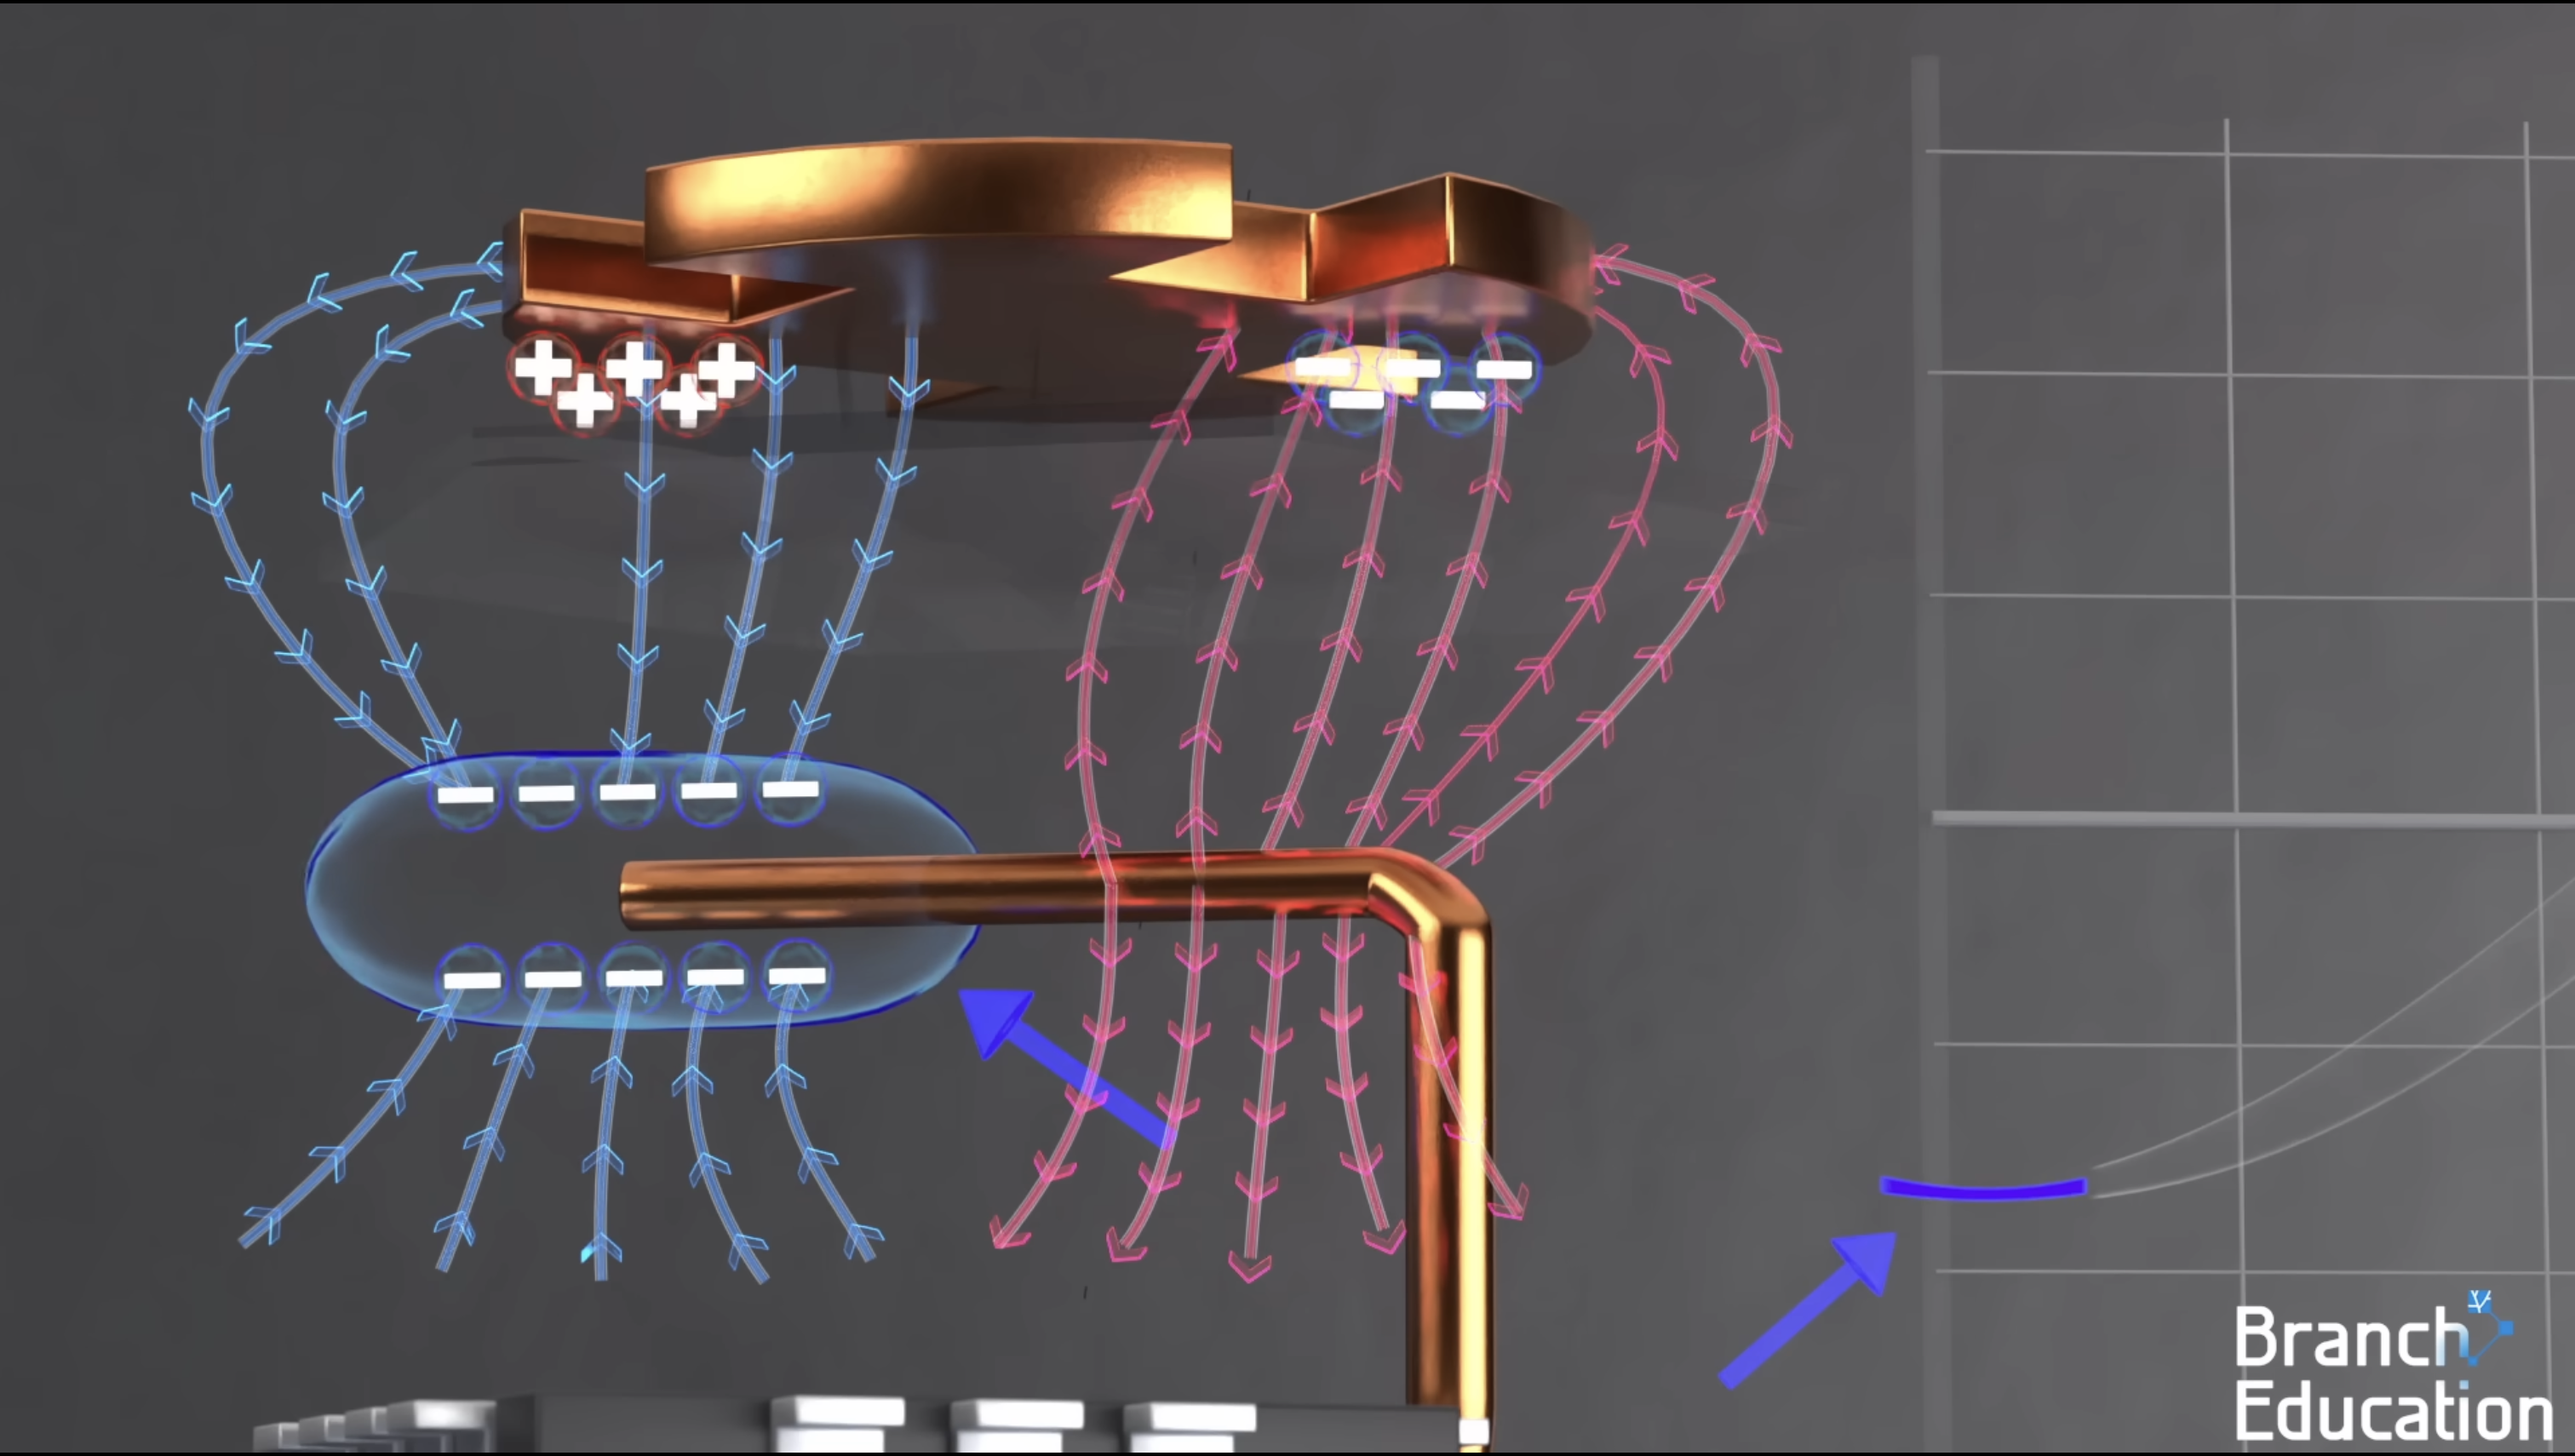
\includegraphics[width=0.8\linewidth]{./res/img/antenna_voltage_applied.png}
  \caption{Aperture Couple Patch antenna con un segnale applicato \cite{branch_education_how_2022}}
  \label{fig:aperture-couple-patch-antenna-voltage-applied}
\end{figure}

Poiché la tensione del filo di alimentazione oscilla con un intervallo di 42 picosecondi tra un picco e un avvallamento, anche i campi elettrici nel patch oscilleranno mentre gli elettroni vanno avanti e indietro.

\begin{figure}[htbp]
  \centering
  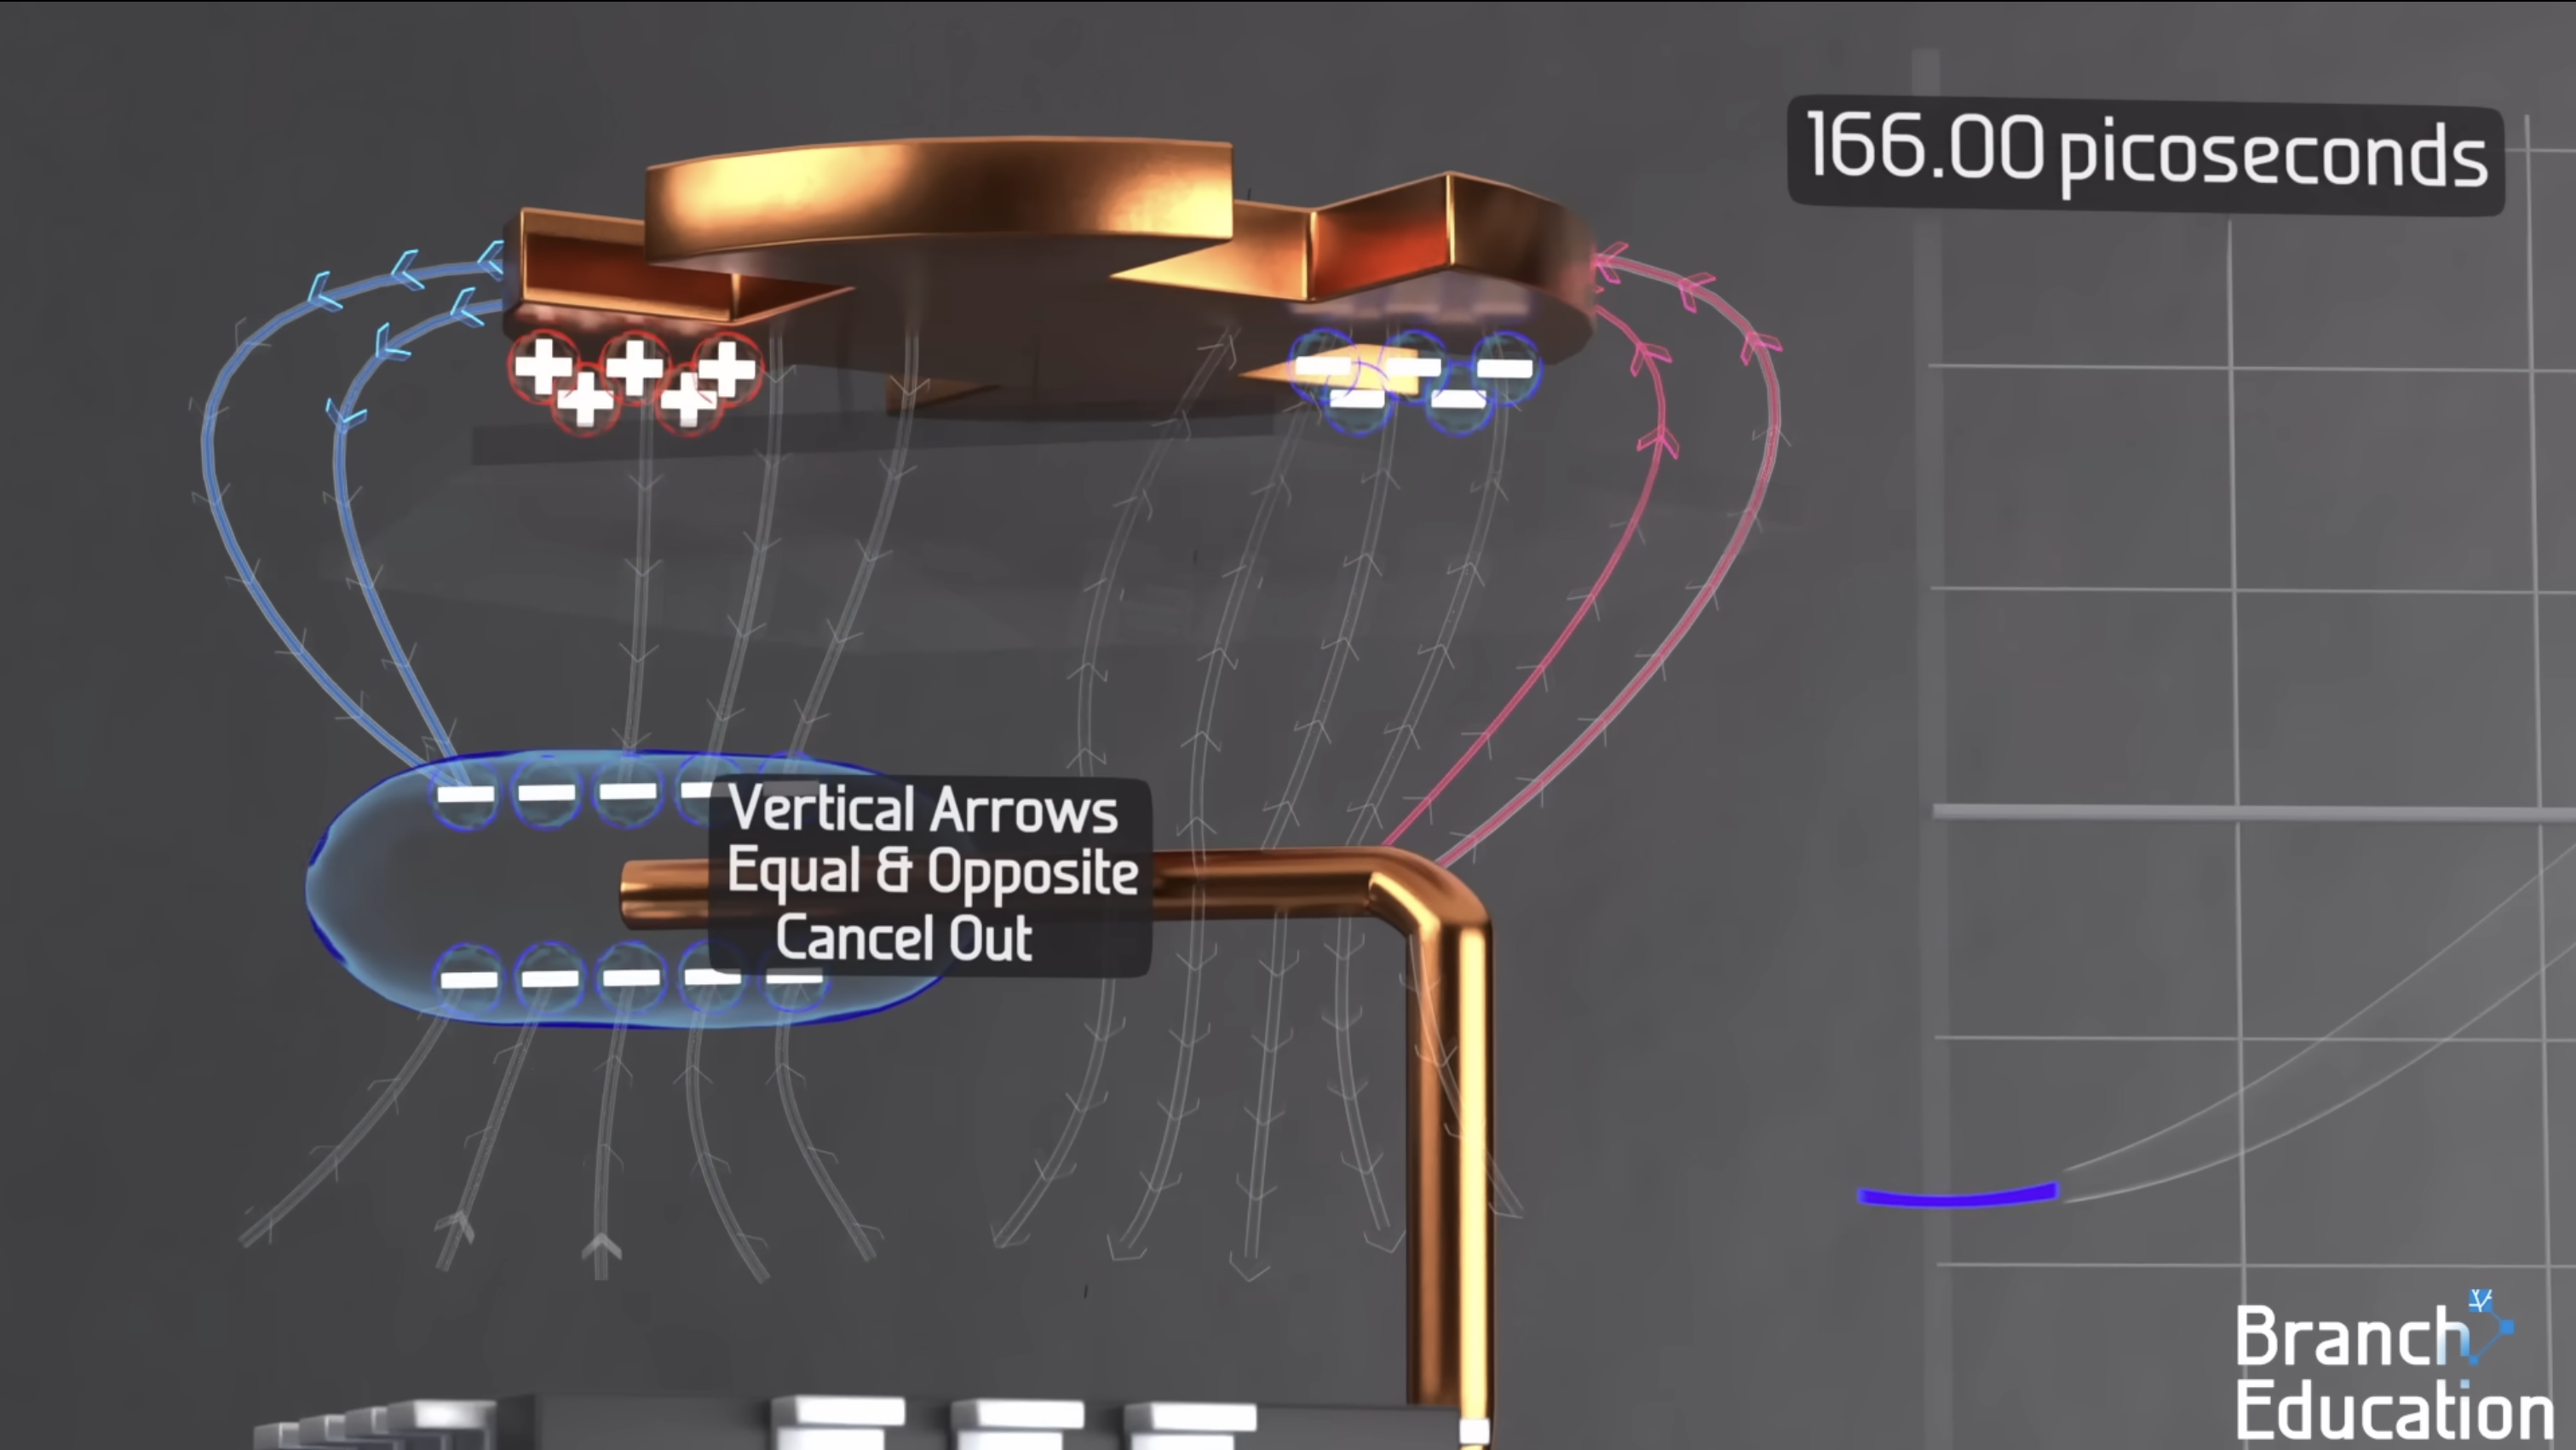
\includegraphics[width=0.8\linewidth]{./res/img/antenna_fringing_fields.png}
  \caption{Creazione dei campi di frangia in un'Aperture Couple Patch antenna \cite{branch_education_how_2022}}
  \label{fig:aperture-couple-patch-antenna-fringing-fields}
\end{figure}

Possiamo vedere in figura \ref{fig:aperture-couple-patch-antenna-fringing-fields} che alcuni di questi vettori di campo elettrico provenienti dal patch sono verticali e, poiché sono uguali e opposti, si annullano.
Tuttavia, altri campi elettrici sono orizzontali nello stesso piano del patch e sono chiamati campi di frangia.
Questi campi di frangia sono nella stessa direzione e quindi si sommano l'uno all'altro, dando luogo a un campo elettrico combinato.\cite{branch_education_how_2022}

Allo stesso tempo, gli elettroni che scorrono da un lato all'altro del disco, che costituiscono una corrente elettrica, generano un campo magnetico con un'intensità e una direzione, o vettore, perpendicolare al vettore del campo elettrico di frangia.
Di conseguenza, abbiamo un campo elettrico orientato in un senso e un campo magnetico orientato perpendicolarmente, come si può vedere in figura \ref{fig:aperture-couple-patch-antenna-em-field}.\cite{branch_education_how_2022}

\begin{figure}[htbp]
  \centering
  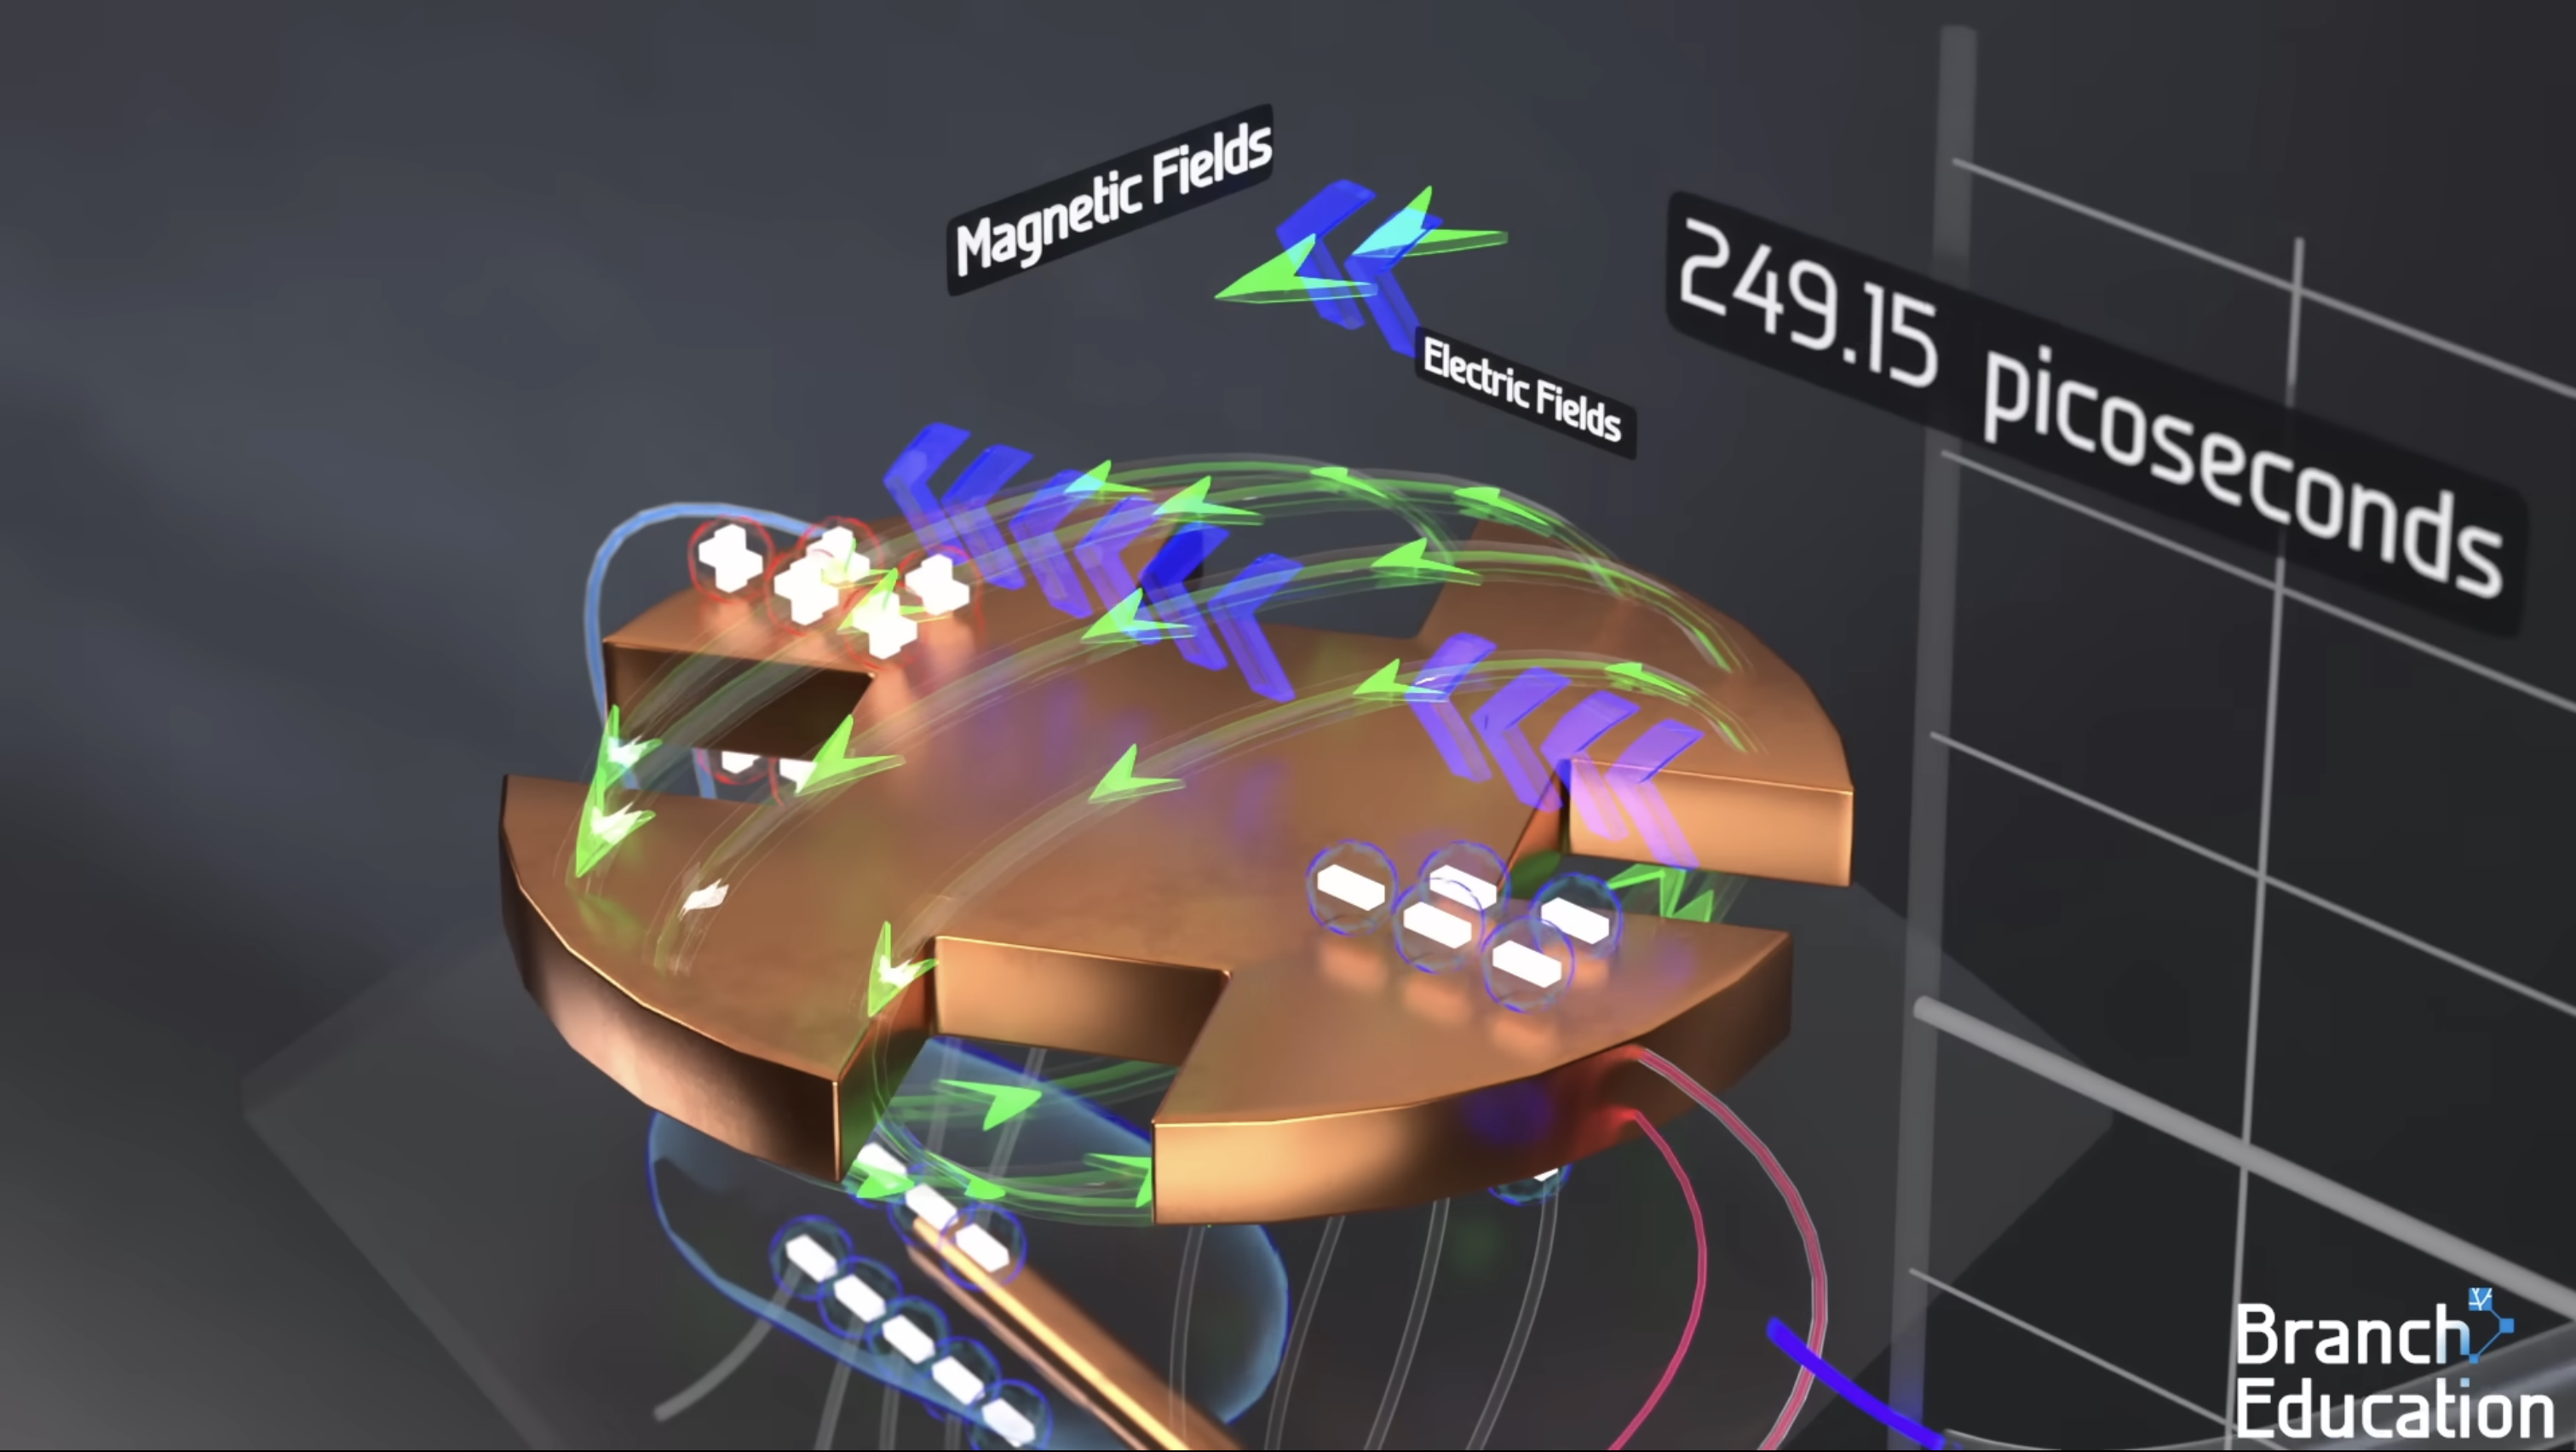
\includegraphics[width=0.8\linewidth]{./res/img/antenna_em_field.png}
  \caption{Campo elettromagnetico in un'Aperture Couple Patch antenna \cite{branch_education_how_2022}}
  \label{fig:aperture-couple-patch-antenna-em-field}
\end{figure}

42 picosecondi dopo, quando la tensione sulla linea di alimentazione diventa positiva, e siamo al picco della sinusoide, la tensione e la corrente sono invertite.
Quindi il campo elettrico e quello magnetico puntano alla direzione opposta.

\subsubsection{Emissione delle onde elettromagnetiche}
Creando i campi elettromagnetici oscillanti vengono generate onde elettromagnetiche che viaggiano in direzione perpendicolare al campo elettrico e al campo magnetico.
Dato che i due insiemi di campi non sono tutti sullo stesso piano, ma sono curvati, l'onda elettromagnetica che si propaga viaggia verso l'esterno in una forma di guscio che si espande.

L'intensità di questi campi è legata direttamente alla tensione che è stata originariamente mandata alla linea di alimentaizone alla base dell'antenna.
Questo significa che se vogliamo rendere questi campi elettromagnetici più intensi basta aumentare la tensione inviata alla linea di alimentazione.

Per ricevere il segnale basta switchare il microchip dell'antenna, chiamato modulo front-end, che si vede in figura \ref{fig:aperture-couple-patch-antenna} da modalità trasmettitore a modalità ricevitore.

TODO: MIGLIORARE SPIEGAZIONE RICEZIONE ONDA ELETTROMAGNETICA

Quando un'onda elettromagnetica dal satellite è diretta verso l'antenna, i campi elettromagnetici del segnale in arrivo influenzano gli elettroni nel patch di rame, generando un flusso di elettroni.

Questo segnale ad alta frequenza ricevuto è inviato alla feedlite dove il modulo di front-end che amplifica il segnale.
Quindi, queste antenne possono essere usate sia per trasmettere che per ricevere onde elettromagnetiche, ma non allo stesso tempo.\cite{branch_education_how_2022}

% COMBINAZIONE DI SINGOLE ANTENNE PER AMPLIFICARE IL SEGNALE
% 11:06/28:08
\subsubsection{Beamforming: come formare un fascio di onde elettromagnetiche che raggiunge lo spazio}
Le tecnica di combinare la potenza delle 1280 antenne in un array esagonale è chiamato beamforming.

Come prima cerchiamo di semplificare il concetto vedendo cosa succede per due antenne affiancate.
Come menzionato prima, un'antenna genera un'onda elettromagnetica che si propaga all'esterno a forma di guscio che si espande.
In ogni singolo punto dello spazio c'è solo un vettore di campo elettrico con un'intensità e una direzione, quindi i vettori di campo elettrico delle due antenne si combinano assieme in tutti i punti nello spazio.
In alcune aree, i campi elettrici delle antenne puntano nella stessa direzione con picchi sovrapposti, e quindi per interferenza costruttiva si sommano.
In altri punti invece sono opposti, con un picco e un'avvallamento, e quindi si cancellano per interferenza distruttiva.

\begin{figure}[htbp]
  \centering
  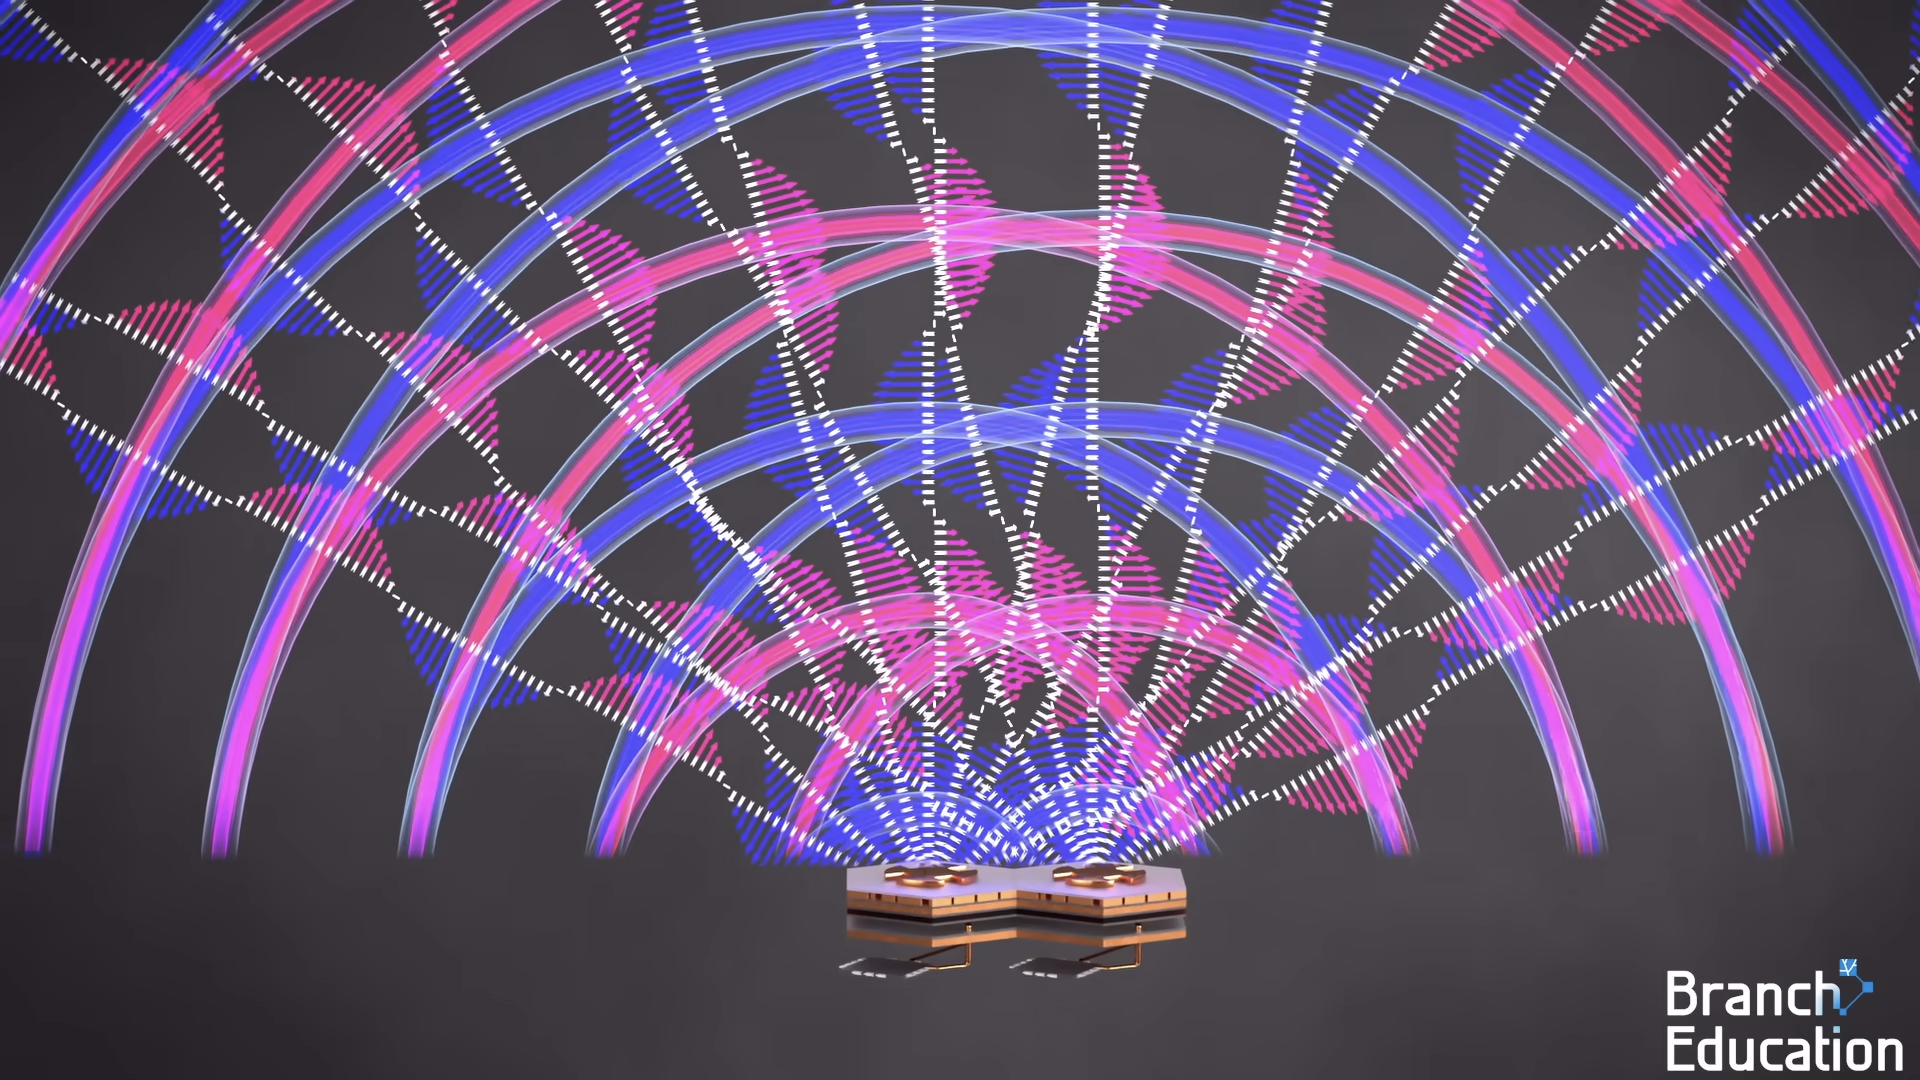
\includegraphics[width=0.8\linewidth]{./res/img/antenna_interference.png}
  \caption{Creazione di interferenze in un array di antenne Aperture Couple Patch \cite{branch_education_how_2022}}
  \label{fig:aperture-couple-patch-antenna-interference}
\end{figure}

Quando aggiungiamo ancora più antenne la zona di interferenza costruttiva diventa ancora più focalizzata rispetto a una singola antenna, in quello che viene chiamato fronte del fascio.
Così, aggiungendo 1280 antenne, possiamo formare un fascio con un'intensità e una direzionalità tali da raggiungere lo spazio.\cite{branch_education_how_2022}

% Ora potreste pensare che la forza di un'antenna duplicata 1280 volte dia luogo a una potenza combinata pari a 1280 volte quella di una singola antenna, ma vi sbagliereste. La potenza e la portata effettive del fascio principale di tutte queste antenne combinate sono in realtà più vicine a 3500 volte quelle di una singola antenna.
% LEGGERE MAIL CORVAJA PER MODIFICARE

\subsubsection{Beam Steering: direzionare un fascio di onde elettromagnetiche}
Come menzionato precedentemente dobbiamo direzionare le onde elettromagnetiche per puntare al satellite starlink che viaggia in \ac{LEO} a 27'000 km/h.
Usare i motori dell'antenna non è abbastanza preciso e creerebbe stress inutile sui motori.
La soluzione è quindi di usare quello che viene chiamato Phased Array Beam Steering.

Torniamo ancora una volta all'esempio delle due antenne.
Prima stavamo inviando lo stesso segnale alle due antenne, e quindi queste erano in fase l'una con l'altra.
Per fare beam steering invece si invia il segnale alle antenne shiftato in fase per poterlo angolare.
Come risultato i tempi dei picchi e delle valli emesse da un'antenna sono differenti dalle altre.
In questo modo le posizioni delle interferenze costruttive sono angolati verso una certa direzione, con interferenze distruttive da tutte le altre parti.
Quindi, cambiando continuamente la fase del segnale inviato all'antenna possiamo creare una zona di sweeping di interferenza costruttiva.

Per sapere l'angolo esatto a cui il fascio di onde deve essere indirizzato si usano le coordinate GPS dell'antenna tramite il suo chip GPS, insieme alle posizioni orbitali del satellite Starlink che è conosciuto nel software dell'antenna.
Il software calcola l'angolo e lo shift di fase richiesto per ciascuna delle antenne.
I risultati dei calcoli del phase shift sono successivamente inviati ai 20 chip più grandi chiamati beamformers, e ciascun beamformer coordina 32 chip più piccoli chiamati moduli di front end, ciascuno dei quali controlla 2 antenne.
Ogni pochi microsecondi questi calcoli sono aggionrati e distribuiti in tutto il PCB dell'antenna in modo da orientare perfettamente il segnale verso il satellite.
Come risultato, il raggio può essere orientato ovunque in un campo visivo di 100 gradi.\cite{branch_education_how_2022}

% FOTO DEL SATELLITE E STRUTTURA
% ci sono 4 antenne nel satellite. Due sono usate per comunicare con multipli terminali utente e le altre 2 sono usate per comunicare con le ground station per trasmettere il traffico internet a terra

\subsubsection{Invio dei dati in un segnale al satellite}
La capacità di un satellite Starlink sarà di 20 Gbit/s quando opererà in due polarizzazioni con modulazione 64-\ac{QAM}.
Ad oggi la rete può usare solo una polarizzazione.
Per lavorare con la 64-\ac{QAM} è necessario avere un \ac{SNR} di più di 17dB.
Al momento questo parametro al terminale UT-1 è tra gli 11 e i 12.5 dB, che corrisponde a una 16-32\ac{APSK} e ha un'efficienza spettrale di 4.5 bit/Hz al massimo.
Le possibili efficienze spettrali per Starlink sono:

\begin{table}[h]
\centering
\begin{tabular}{|c|c|c|c|}
\hline
\textbf{Modulation} & \textbf{Code rate} & \makecell{\textbf{Spectral efficiency}\\ \textbf{bit/s/Hz}} & \makecell{\textbf{Spectral efficiency} \\ \textbf{dB}}\\ \hline
QPSK     & 0.5   & 0.989  & -0.05 \\ \hline
8PSK     & 0.75  & 2.228  & 3.48  \\ \hline
8PSK     & 0.833 & 2.479  & 3.94  \\ \hline
16APSK   & 0.666 & 2.637  & 4.21  \\ \hline
16APSK   & 0.75  & 2.967  & 4.72  \\ \hline
32APSK   & 0.9   & 4.453  & 6.49  \\ \hline
64QAM    & 0.772 & 4.5234 & 6.55  \\ \hline
64QAM    & 0.873 & 5.1152 & 7.09  \\ \hline
64QAM    & 0.948 & 5.5547 & 7.45  \\ \hline
\end{tabular}
\caption{Efficienza spettrale di Starlink \cite{rozenvasser_estimation_2023}.}
\end{table}

\paragraph{Link budget}
La potenza ricevuta al terminale utente è data da:
\begin{equation}
P_{rx} = P_{tx} + G_{tx} + G_{rx} - L_{tx} - L_{rx} - L_{atm} - L_{p}
\label{eq:received-power}
\end{equation}

In questa equazione, $P_{tx}$ è la potenza del trasmettitore, $G_{tx}$ e $G_{rx}$ sono i guadagni del trasmettitore e del ricevitore, $L_{tx}$ e $L_{rx}$ sono le perdite ai trasmettitori e ricevitori, $L_{atm}$ è la perdita atmosferica, e $L_{p}$ è il path loss introdotto dalla separazione tra il trasmettitore e il ricevitore.

$P_{tx}$ è la potenza del trasmettitore ed è dipendente dall'allocazione dinamica delle risorse $\eta_{a}$ e massa del satellite $m$.

Il guadagno del trasmettitore $G_{tx}$ è dipendente dalla tecnologia dell'antenna (il diametro $d$ e la lunghezza d'onda $\lambda$):
\begin{itemize}
  \item Parabolica: $G_{tx} = 20 * \log_{10} (\frac{\eta_{a} \pi d}{\lambda})$
  \item Phased Array: $G_{tx} = 20 * \log_{10} (\frac{4 \eta_{a} \pi \sqrt[3]{m^2}}{\lambda})$
\end{itemize}

Il guadagno del ricevitore sul rumore $G_{rx}$ basato sul tipo del terminale utente:
\begin{itemize}
  \item Parabolica: $G_{rx} = 5.24 dB$
  \item Phased Array: $G_{rx} = 10.8 dB$
\end{itemize}

La perdita atmosferica $L_{atm}$ è dipendente dalla banda di frequenza e pressione atmosferica $P_{atm}$.
Per la Ku/Ka-band $L_{atm} = 0.97 dB/km$ in media.

\begin{figure}[htbp]
  \centering
  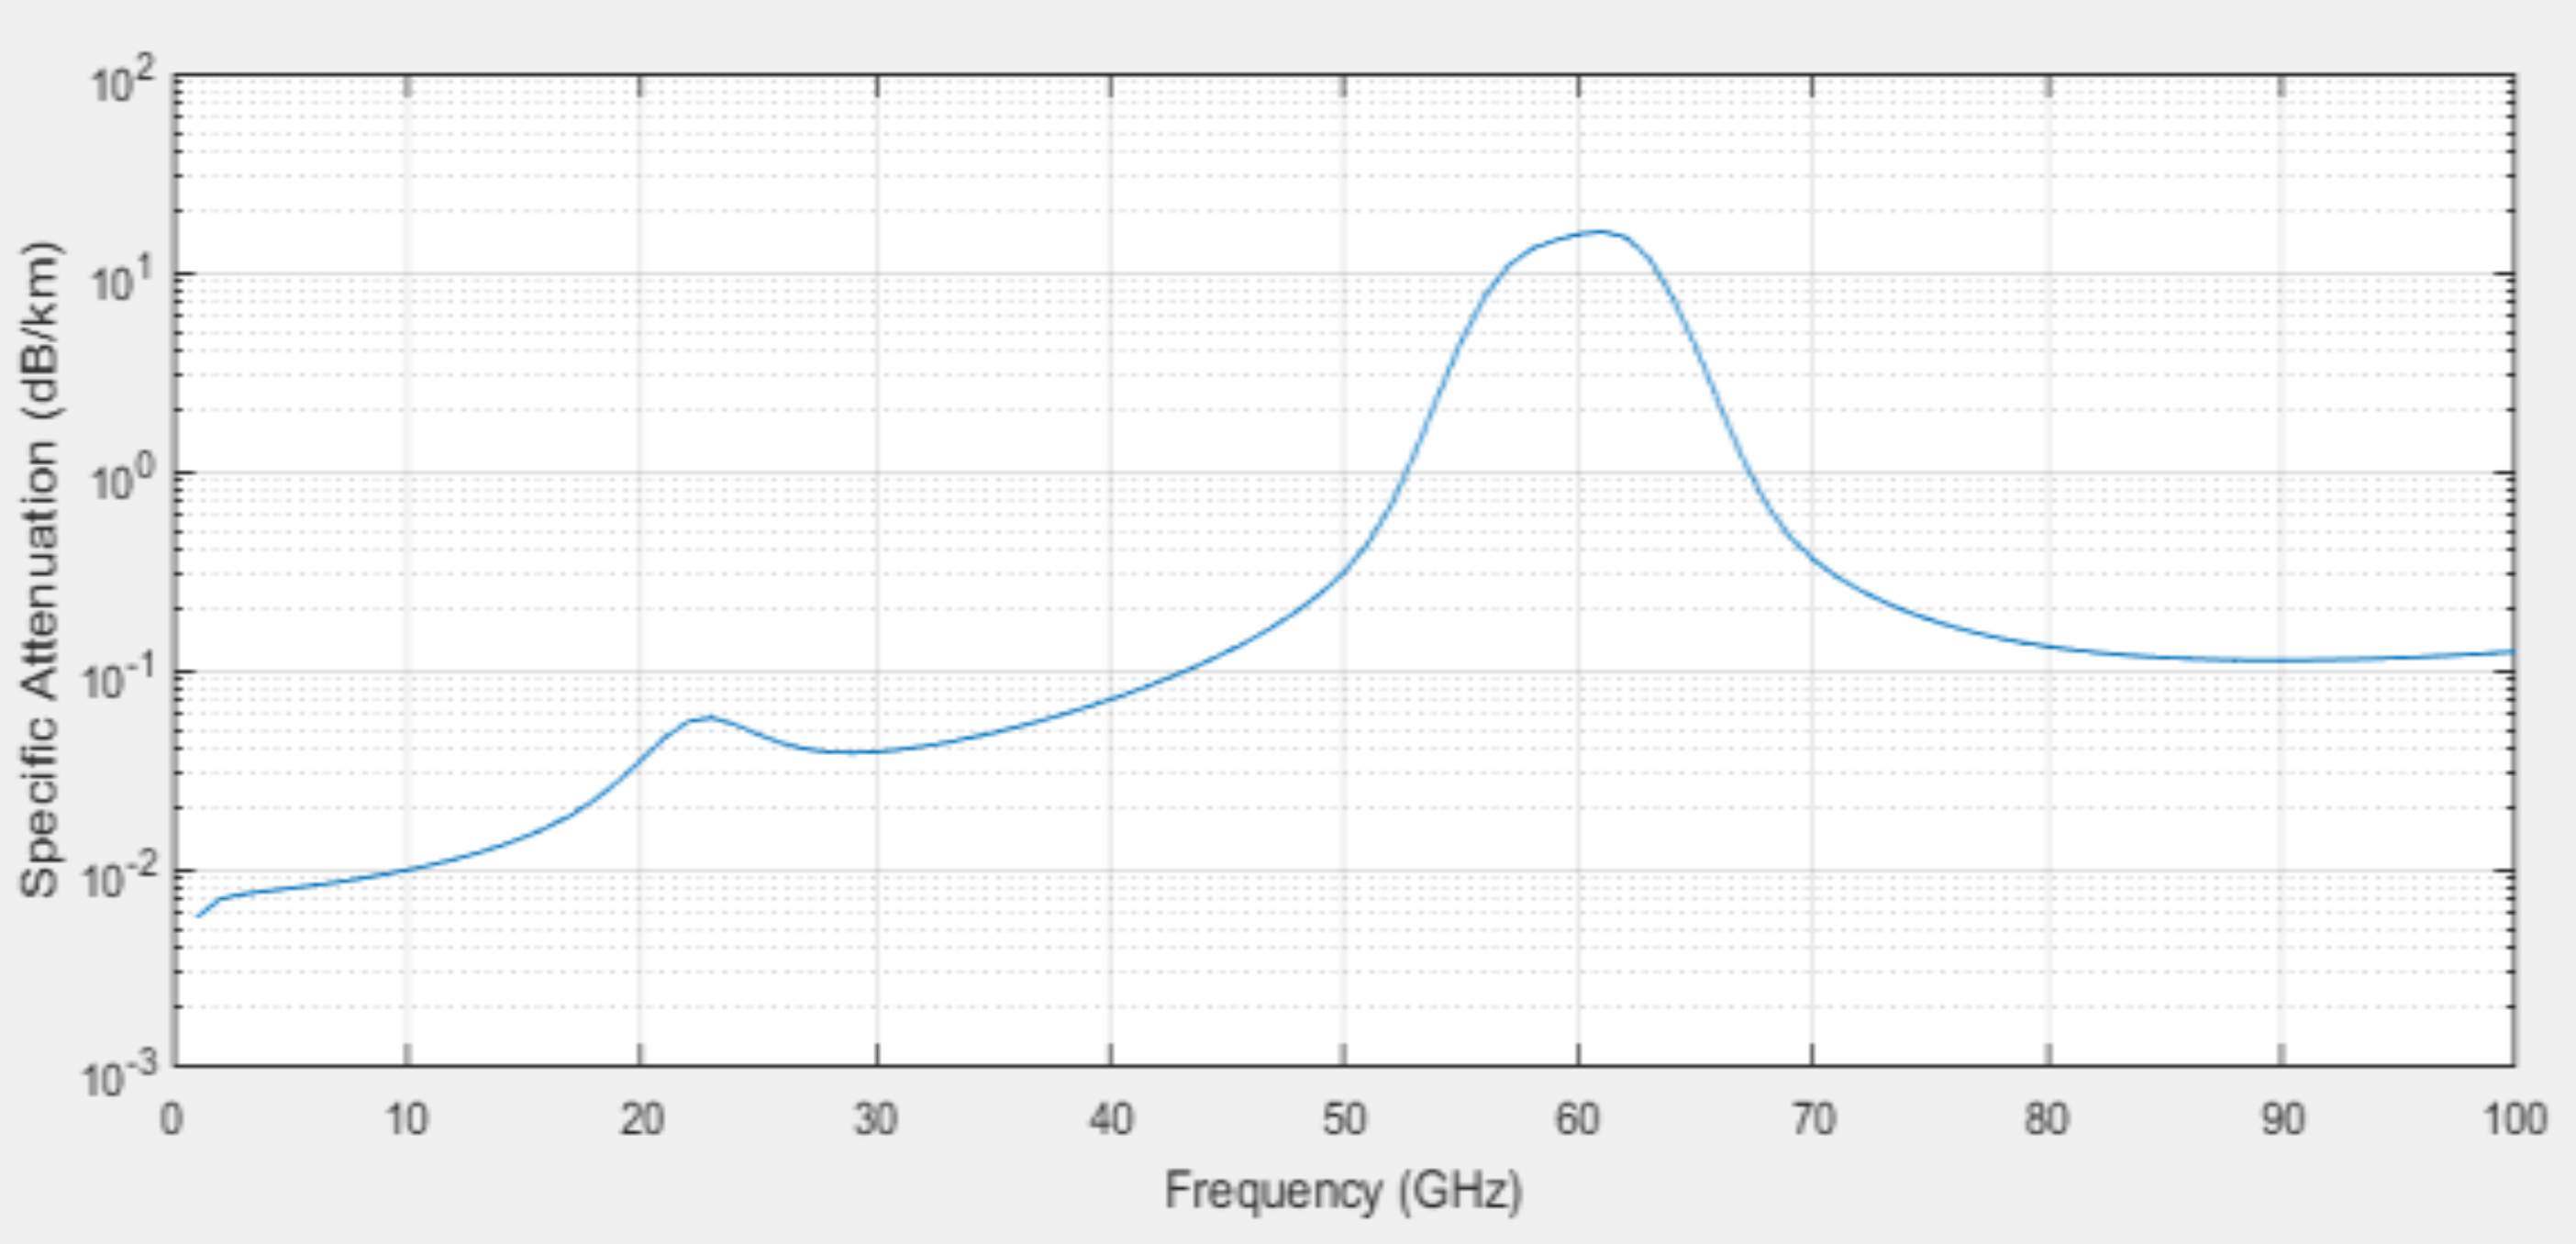
\includegraphics[width=0.8\linewidth]{./res/img/atmospheric_losses_simulation.png}
  \caption{Simulazione delle perdite atmosferiche}
  \label{fig:atmospheric-losses-simulation}
\end{figure}

Osserviamo in figura \ref{fig:atmospheric-losses-simulation} un picco del parametro $L_{atm}$ a 60 GHz.
Per ridurre l'influenza delle perdite atmosferiche è preferibile usare i range di frequenza fino a 53 GHz, che corrisponde al piano di frequenze proposto da SpaceX (tabella \ref{tab:starlink-frequency-allocation-modulation-type})
Per la trasmissione in uplink si usano le frequenze 14-52.4 GHz e per la trasmissione in downlink le frequenze 10.7-42.5 GHz.
Nella tabella \ref{tab:starlink-frequency-allocation-modulation-type} possiamo anche vedere i tipi di modulazione.
Il tipo di modulazione può cambiare da \ac{BPSK} a 64-\ac{QAM}.

\begin{table}[h]
\centering
\begin{tabular}{|c|c|c|}
\hline
\textbf{Caratteristica} & \textbf{Uplink} & \textbf{Downlink} \\ \hline
Frequenza (GHz)  & \makecell{14.0-14.5 \\ 27.5-29.1 \\ 29.5-30.0 \\ 47.2-52.4}  & \makecell{10.7-12.7\\17.8-18.6\\18.8-19.3\\37.5-42.5} \\ \hline
Tipo di modulazione  & \makecell{\ac{BPSK},\\M\ac{QAM}} & \makecell{\ac{OQPSK},\\M\ac{QAM}} \\ \hline
\end{tabular}
\caption{Path loss nello spazio aperto in dB ($L_p$) \cite{rozenvasser_estimation_2023}.}
\label{tab:starlink-frequency-allocation-modulation-type}
\end{table}

$L_p = 20 * \log_{10} (\frac{4 \pi d}{\lambda})$

\begin{figure}[htbp]
  \centering
  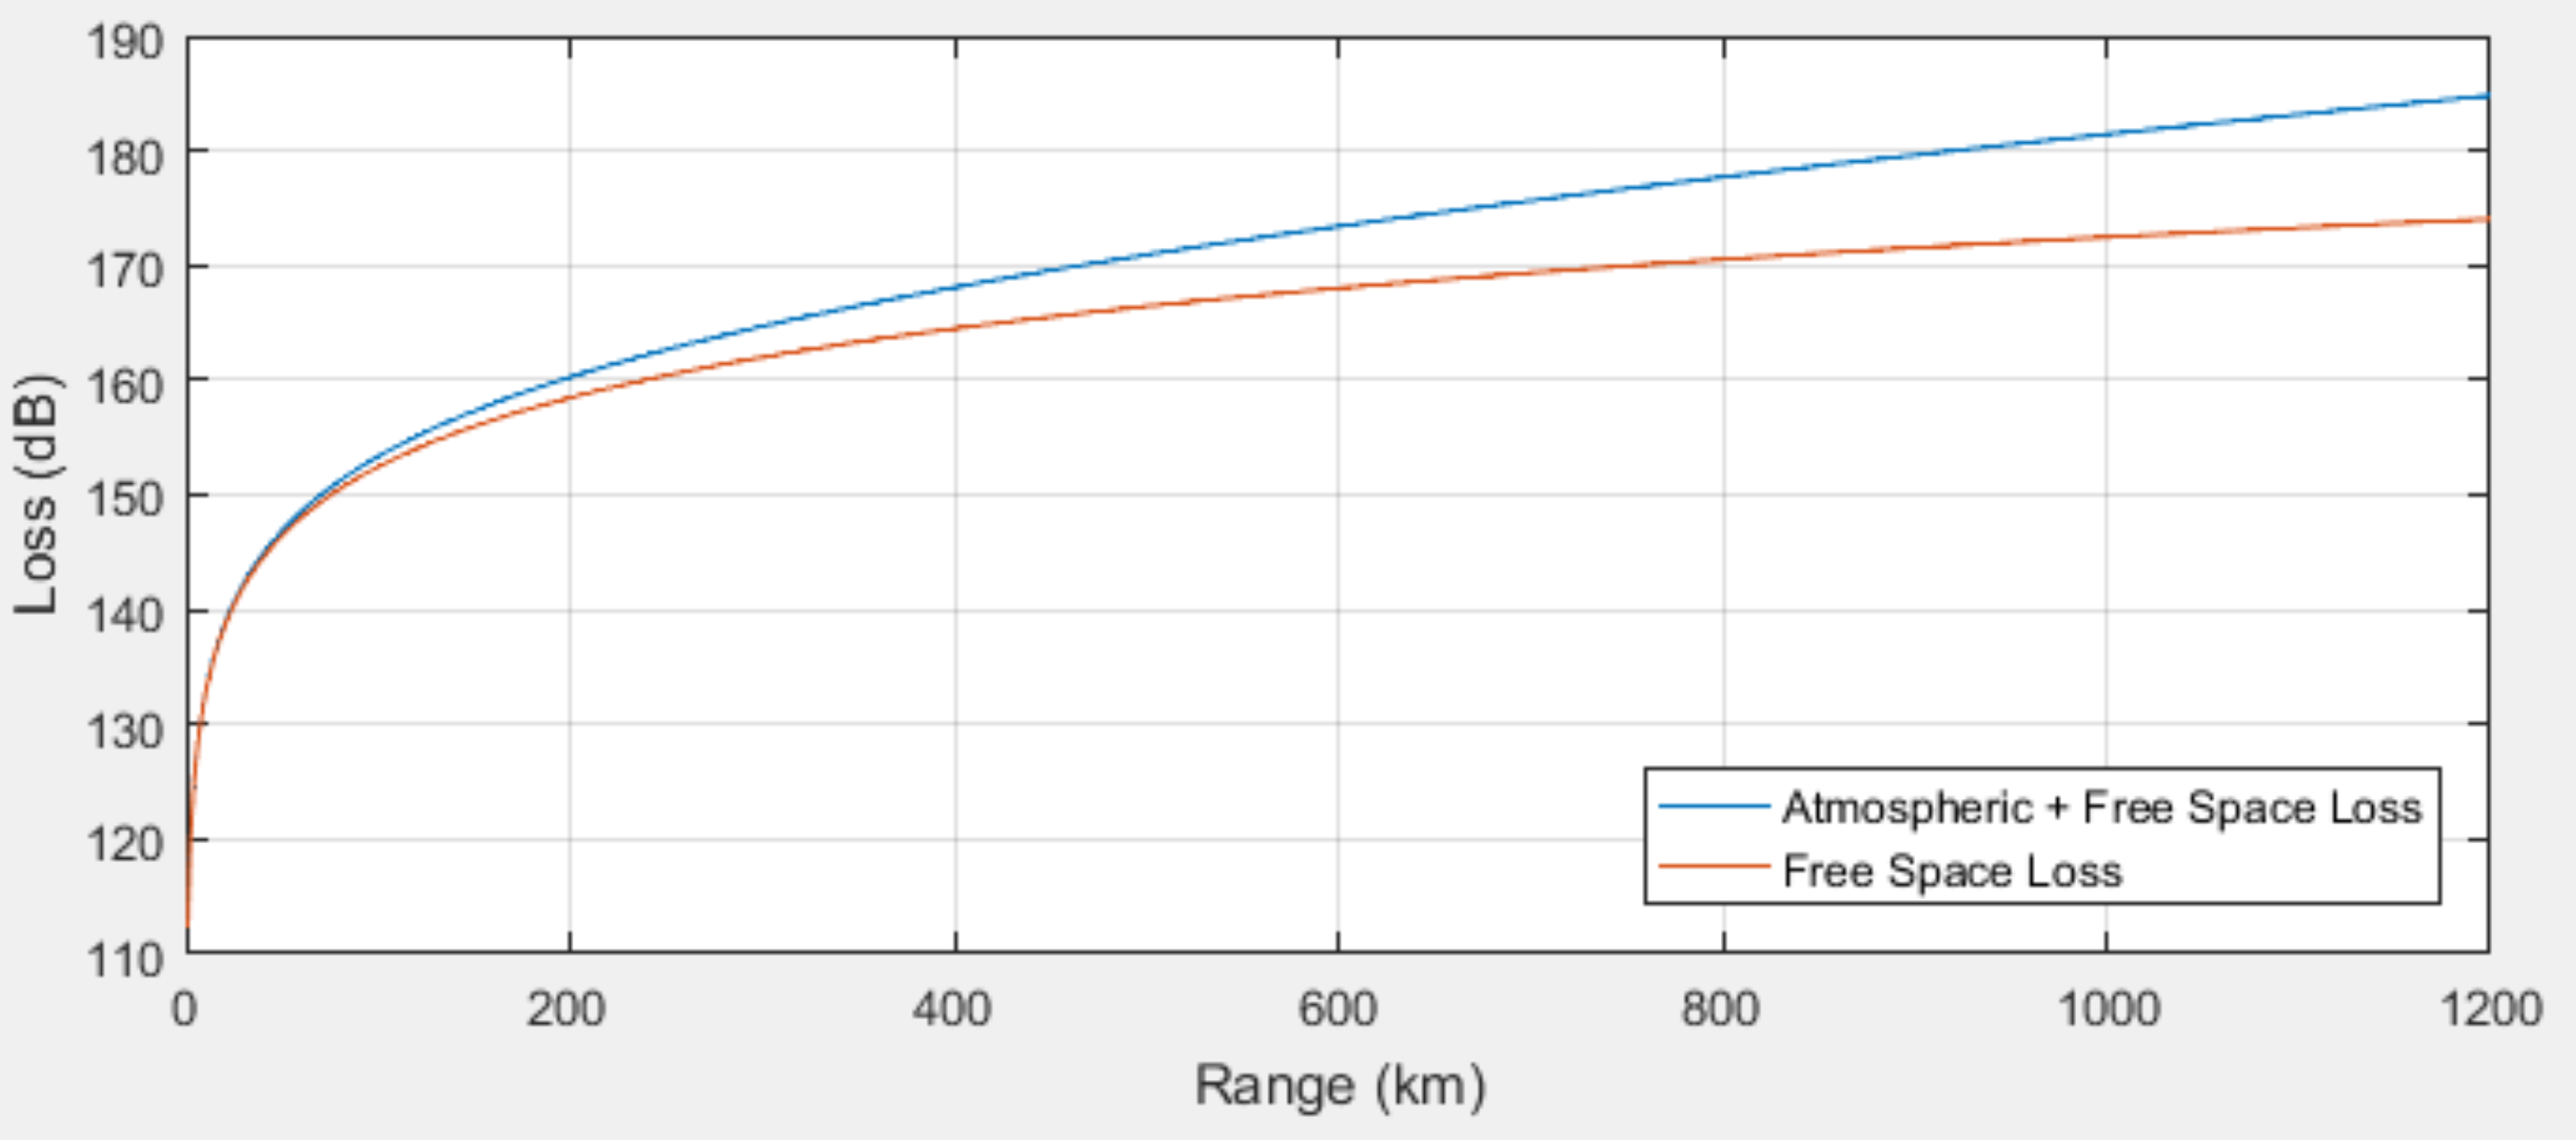
\includegraphics[width=0.8\linewidth]{./res/img/free_space_path_loss_atm_loss.png}
  \caption{Path loss nello spazio libero e perdita atmosferica}
  \label{fig:free-space-path-loss-atm-loss}
\end{figure}

Il path loss nello spazio libero è il contributore principale alla perdita di potenza come si vede in figura \ref{fig:free-space-path-loss-atm-loss}.
Alle altitudini calcolate per i satelliti Starlink, questo valore è di 160-175 dB.
La perdita totale dal path loss nello spazio libero e le perdite atmosferiche sono 165-185 dB.

I risultati della modellazione e del calcolo della dipendenza della potenza ricevuta dal terminale utente dall'altezza dell'orbita del satellite per varie frequenze (da 10 a 50 GHz) sono illustrati nella figura \ref{fig:link-budget-wo-ecc}.

\begin{figure}[htbp]
  \centering
  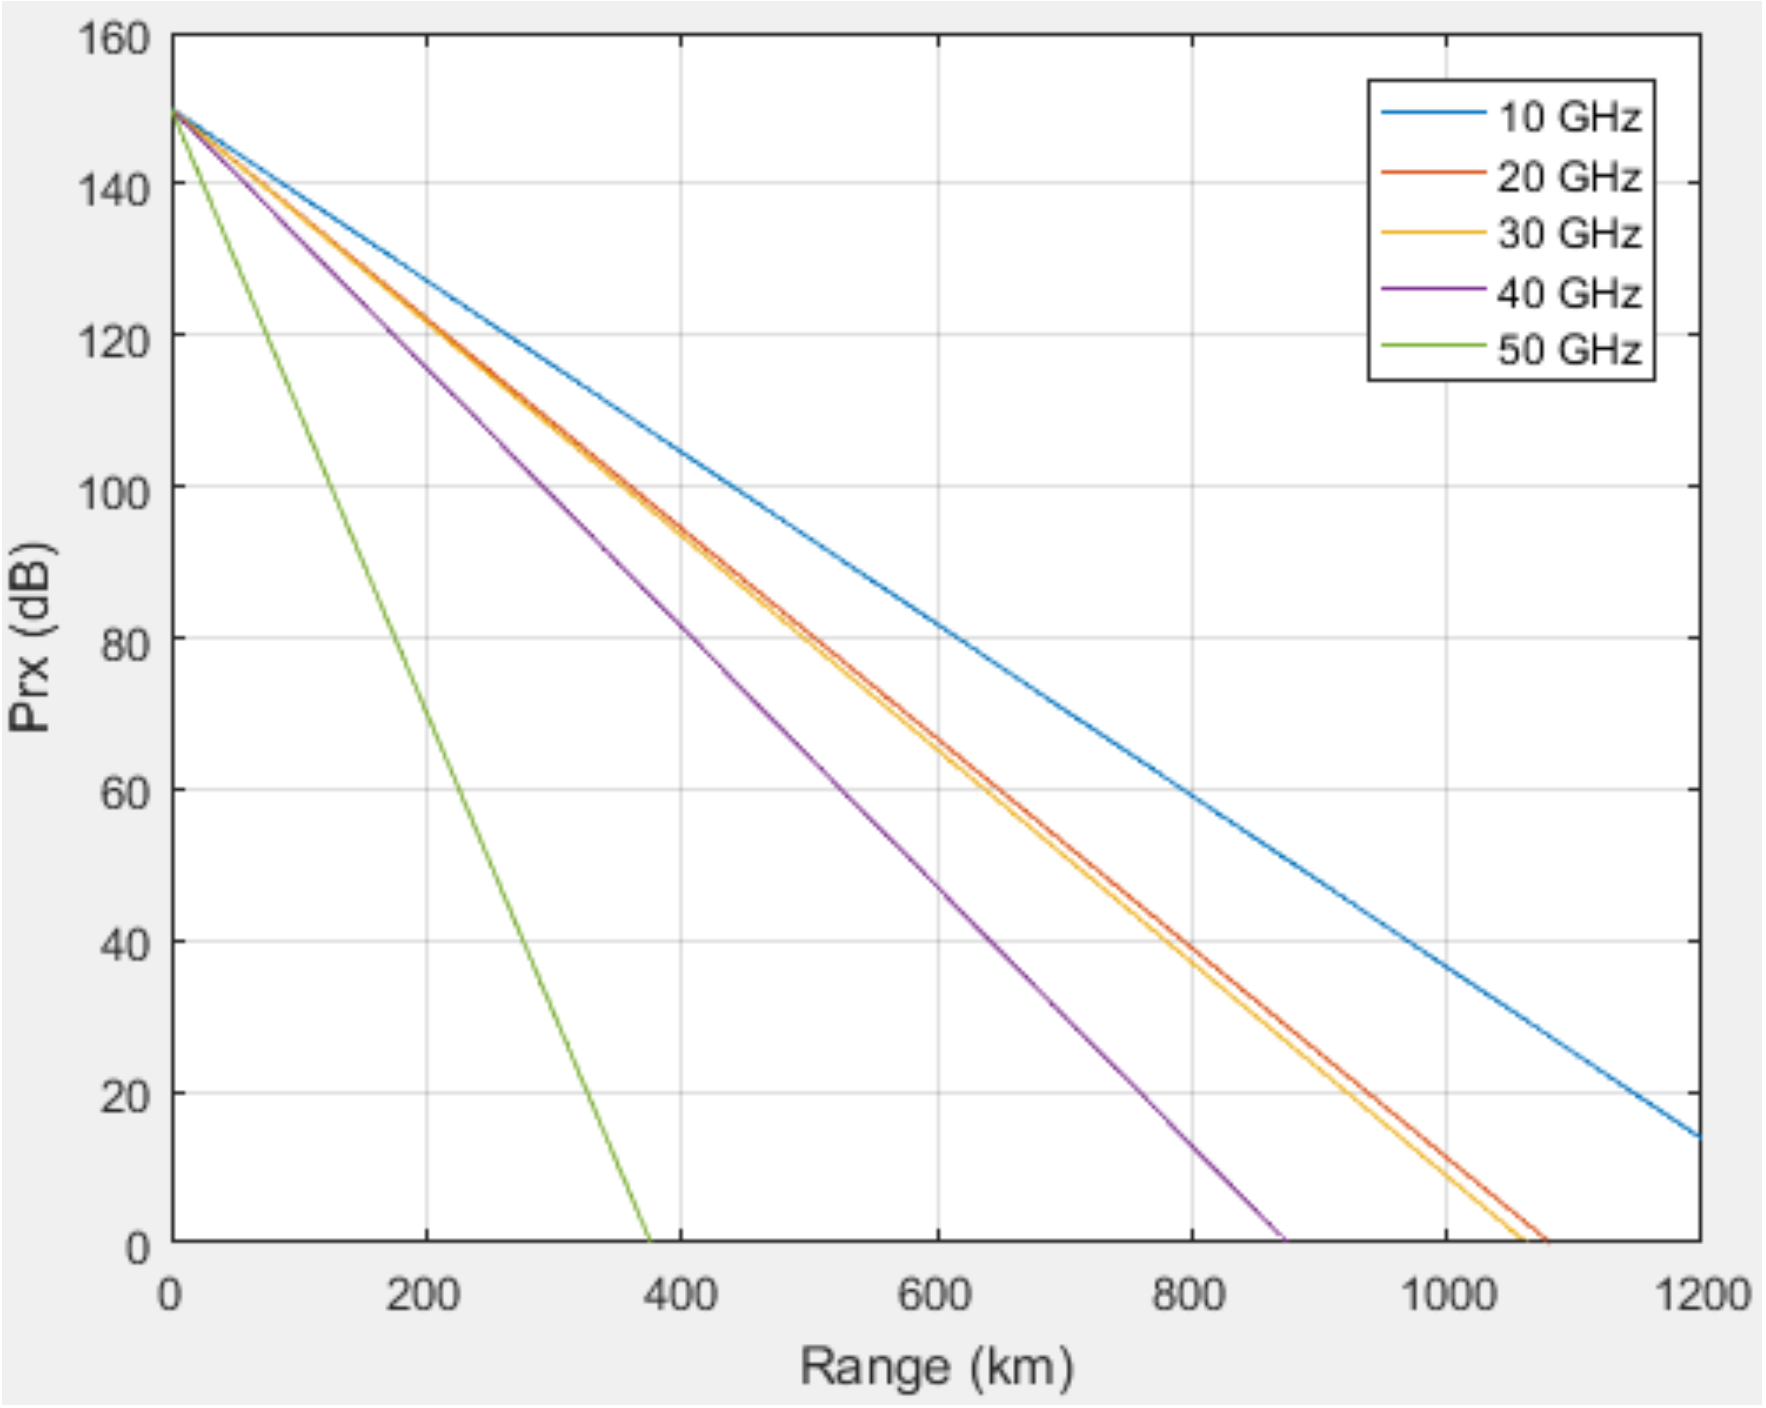
\includegraphics[width=0.8\linewidth]{./res/img/link_budget_wo_ecc.png}
  \caption{Link budget without \ac{ECC}}
  \label{fig:link-budget-wo-ecc}
\end{figure}

Dalla figura \ref{fig:link-budget-wo-ecc} si può vedere che il valore più alto della potenza del segnale è 150 dB.
Finchè il segnale passa attraverso l'atmosfera gradualmente viene attenuato.
L'attenuazione avviene anche sui dispositivi ricevitori e trasmettitori.
Il grado di attenuazione dipende da molti parametri e limita l'altezza dell'orbita del satellite.

È consuetudine utilizzare un codice a correzione di errore per aumentare l'immunità al rumore dei sistemi.
In questo caso, utilizziamo un codice a correzione di errore per aumentare il link budget.

Aggiungiamo CG, guadagno di codifica dovuto al codice a correzione d'errore (\ac{ECC}), all'equazione (\ref{eq:received-power}) che diventa quindi:

\begin{equation}
  P_{rx} = P_{tx} + G_{tx} + G_{rx} - L_{tx} - L_{rx} - L_{atm} - L_{p} + CG
\end{equation}

I risultati della modellazione e calcolo della dipendenza della potenza ricevuta al termianle utente all'altezza dell'orbita del satellite per frequenze diverse (dai 10 ai 50 GHz), considerando l'uso di un codice di correzione di errore con un guadagno di codice di 10 dB è mostrato in \ref{fig:link-budget-w-ecc}

\begin{figure}[htbp]
  \centering
  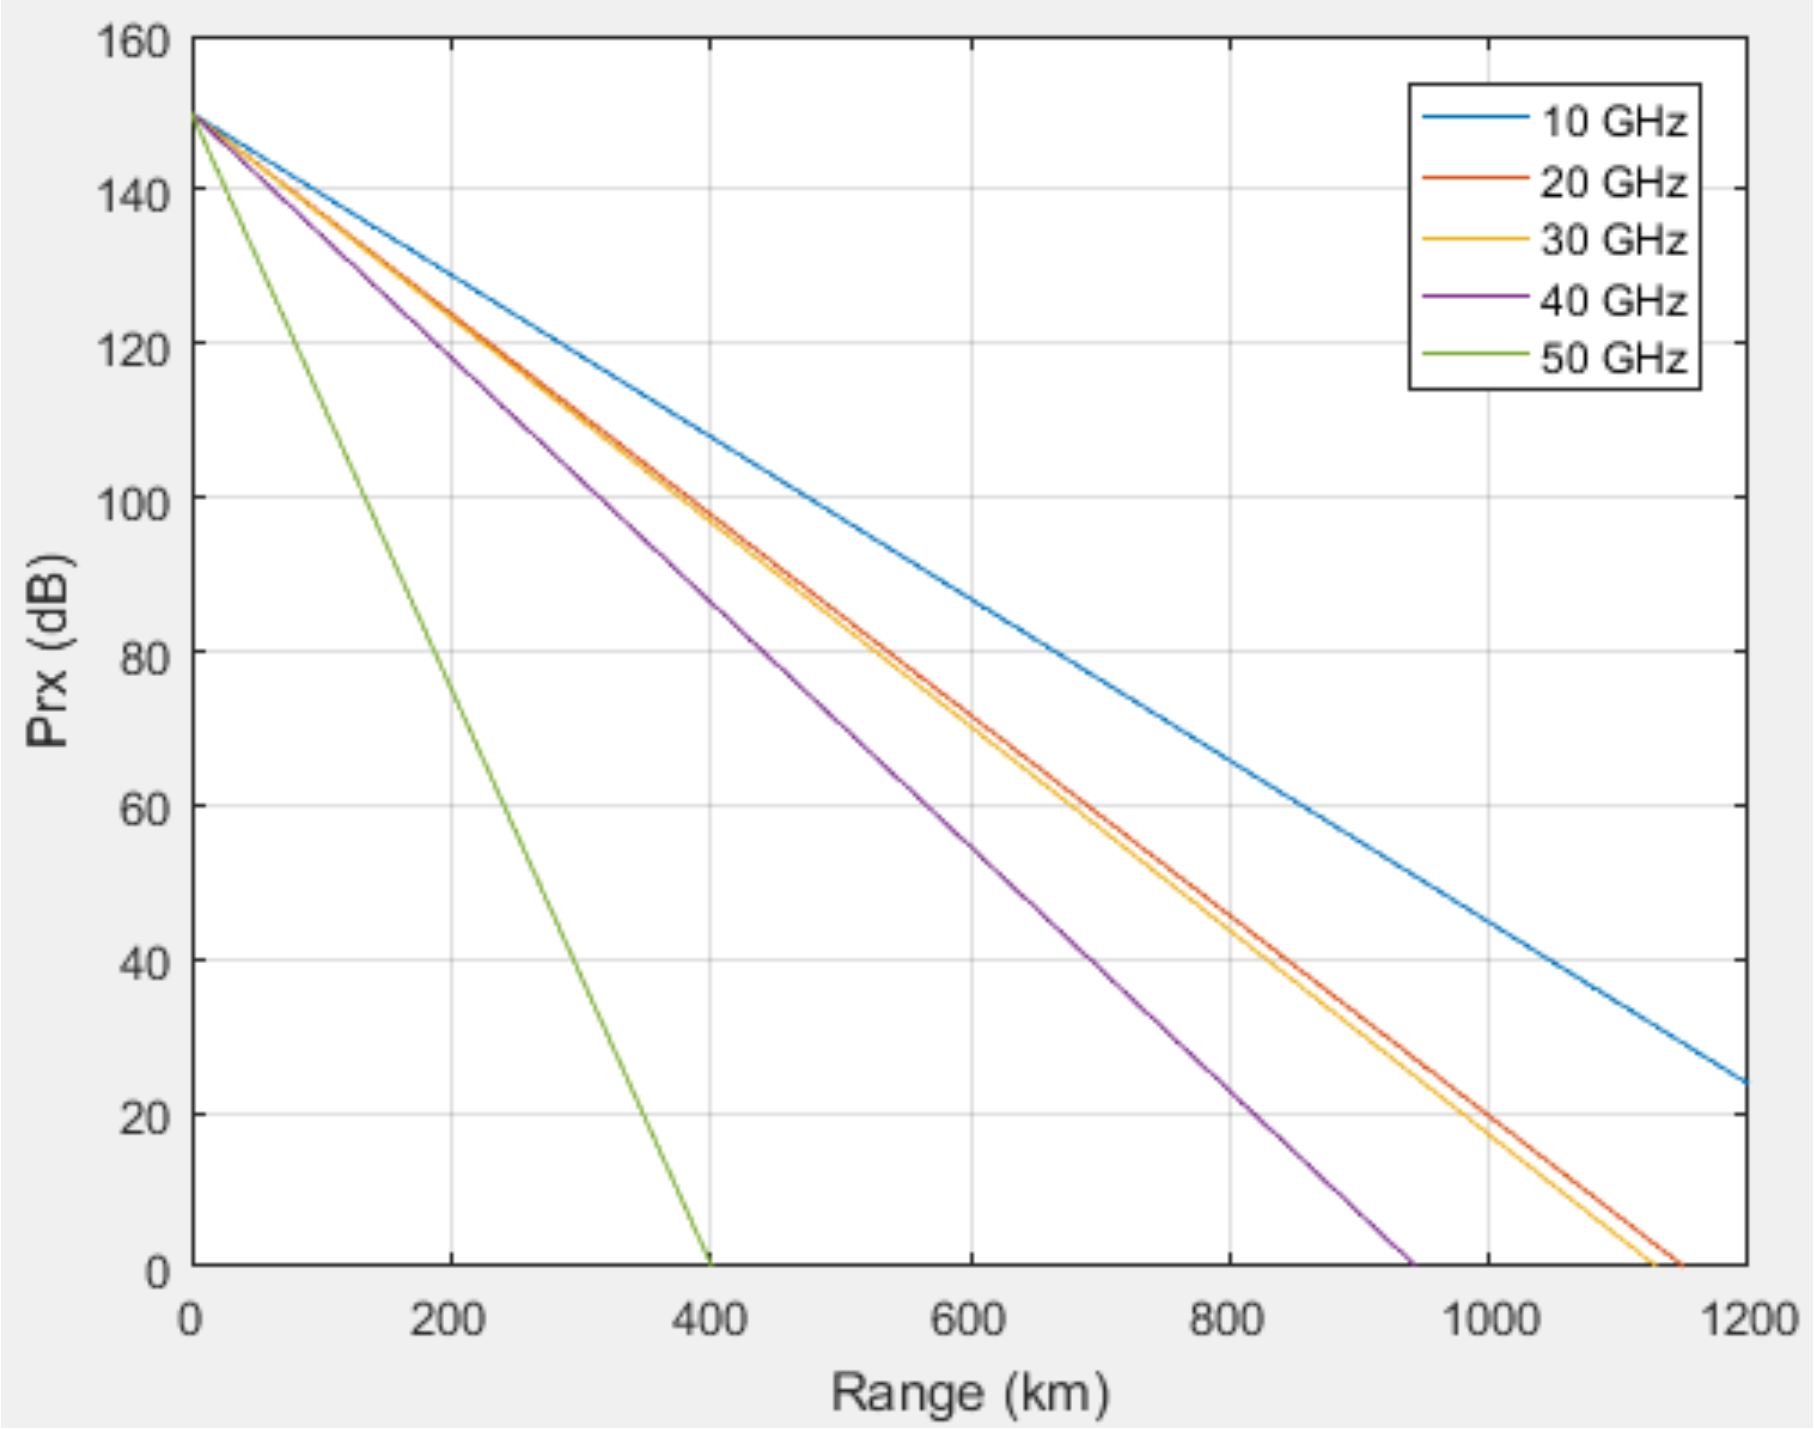
\includegraphics[width=0.8\linewidth]{./res/img/link_budget_w_ecc.png}
  \caption{Link budget without \ac{ECC}}
  \label{fig:link-budget-w-ecc}
\end{figure}

Per assicurare la minima probabilità d'errore è necessario avere un margine del \ac{SNR} al ricevitore, che dipende dal tipo di modulazione.
Dalla figura \ref{fig:link-budget-w-ecc} possiamo vedere che ad alte frequenze l'altezza dell'oribita è limitata a 340 km.
Il lancio della maggior parte dei satelliti è pianificata a quest'altezza.
Per frequenze più basse, possono essere utilizzate orbite più alte a 550 km e 1110 km \cite{rozenvasser_estimation_2023}.

